% for 16x9 (modern wide screen) aspect ratio slides
\documentclass[aspectratio=169]{beamer}

% Oxford Maths theming
\usetheme{oxfordmaths}
\usepackage{xcolor}

% Drop the infolines headline (section/subsection name above each frame title)
\setbeamertemplate{headline}{}

% ===== Semantic color palette =====
% Observed data (empirical / from experiment)
\colorlet{colData}{green!20}
\colorlet{colDataLine}{green!50!black}
% ODE / differentiable modules
\colorlet{colODE}{blue!12}
\colorlet{colODELine}{blue!70!black}
% Stochastic / simulation modules
\colorlet{colSim}{orange!12}
\colorlet{colSimLine}{orange!70!black}
% Posteriors / inference output
\colorlet{colPost}{violet!15}
\colorlet{colPostLine}{violet!70!black}
% Corner-plot series, as exact hex matches to plot_bursty_boundary.py. The
% legend chips on the results slides are drawn in these, so if the palette
% constants in that script move, move these with them or the chips start lying.
\definecolor{figDiff}{HTML}{3B7EA1}    % differentiable block's own posterior
\definecolor{figAlone}{HTML}{D2762B}   % regulator inferred alone
\definecolor{figCond}{HTML}{3D9970}    % conditioned across the boundary
\definecolor{figTruth}{HTML}{E5007D}   % ground truth
% Infrastructure / neutral
\colorlet{colNeutral}{gray!15}
% Problems / no-UQ / fragile
\colorlet{colWarn}{red!15}
\colorlet{colWarnLine}{red!70!black}

% Free (inferred) parameter in an equation: recolour the symbol itself, so the
% maths spacing is untouched. Works in or out of math mode.
\newcommand{\freeparam}[1]{\ensuremath{{\color{burntorange}#1}}}

\hypersetup{colorlinks=true, urlcolor=teal, linkcolor=., filecolor=.}
%\titlelogo{assets/macsys_logo.png}

% Set author etc info
\title[InferCell]{InferCell: Inference-First Whole-Cell Modelling}
\author{Tom Kimpson}
\institute{University of Melbourne}
\date[2026]{MACSYS ISAB Meeting, 12 August 2026}

% ===== Packages & helpers =====
\usepackage{amsmath, amssymb, mathtools}
\usepackage{booktabs}
\usepackage{siunitx}
\usepackage{tikz}
\usepackage{pgfplots}
\pgfplotsset{compat=1.18}
\usepgfplotslibrary{fillbetween}
\usetikzlibrary{arrows.meta, positioning, calc, decorations.pathreplacing, shapes.geometric, fit}
\usepackage{graphicx}
\graphicspath{{../}}
\usepackage{colortbl}
\usepackage{listings}

% Pre-define TikZ styles
\tikzset{
	modbox/.style={draw, rounded corners=4pt, minimum height=0.9cm, minimum width=2.2cm, font=\small, thick},
	inferbox/.style={draw, rounded corners=4pt, minimum height=0.7cm, font=\footnotesize, dashed, thick},
	pipelinebox/.style={draw, rounded corners, minimum height=0.8cm, font=\small, fill=#1},
	pipelinearr/.style={->, thick, >=stealth},
	brace/.style={decorate, decoration={brace, amplitude=6pt}},
}

% Julia code listing style
\lstdefinestyle{julia}{
	language=Python, % close enough for keywords
	basicstyle=\ttfamily\scriptsize,
	keywordstyle=\color{blue!70!black}\bfseries,
	stringstyle=\color{green!50!black},
	commentstyle=\color{gray},
	showstringspaces=false,
	columns=fullflexible,
	morekeywords={struct, function, end, using, abstract, type},
}

% Reduce cluttered bullets
\setbeamertemplate{itemize items}[circle]
\setbeamertemplate{enumerate items}[default]

% Backup slide commands to exclude appendix from total count
\newcommand{\backupbegin}{
	\newcounter{framenumberappendix}
	\setcounter{framenumberappendix}{\value{framenumber}}
}
\newcommand{\backupend}{
	\setcounter{framenumber}{\value{framenumberappendix}}
}

% Page number template
\makeatletter
\setbeamertemplate{page number in head/foot}{%
	\insertframenumber
}
\makeatother


\begin{document}

% ===== Title =====
\begin{frame}[plain]
	\titlepage
	% Prior/posterior sketch at right, as on the 2026-05 Brisbane MACSYS title slide.
	% Overlaid rather than passed to \titlelogo so the MACSYS logo keeps that slot.
	\begin{tikzpicture}[remember picture, overlay]
		\node[anchor=east, inner sep=0pt]
			at ([xshift=-6mm, yshift=-12mm]current page.east)
			{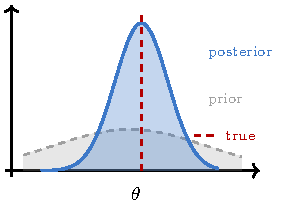
\includegraphics[width=\dimexpr\paperwidth/3\relax]{assets/posterior_plot.pdf}};
	\end{tikzpicture}
\end{frame}




% ================================================================
% SECTION 1: The Problem
% ================================================================
\section{The Problem}



% ----------------------------------------------------------------
\begin{frame}{Whole-Cell Models are Forward Simulators}
	\small
	\begin{itemize}\itemsep2pt
		\item Representative SOTA: the Luthey-Schulten lab's 4D minimal cell --- 493 genes,
		four coupled solvers, 10\,nm voxels, a full cell cycle on GPU
		(\href{https://www.cell.com/cell/fulltext/S0092-8674(26)00174-1}{Thornburg et al., \textit{Cell} 2026}).
		\item Structurally a \textbf{forward simulator}: parameters in, predictions out,
		no uncertainty propagated.
	\end{itemize}

	\vspace{1mm}
	% Column widths = figure width + equal padding, so the three figures sit on
	% an even rhythm (~1.26cm outer margins and gaps). Needs onlytextwidth:
	% without it the block bleeds into the page margins and adds its own glue.
	\begin{columns}[c,onlytextwidth]
		\begin{column}{0.3225\textwidth}
			\centering
			% Coordinates in cm, no scale= key: TikZ scales positions but not node
			% minimum heights, so the old scale=0.62 shrank the 1.6cm pitch to
			% 0.99cm against 0.8cm-tall boxes and left 2mm of arrow. A 1.4cm pitch
			% gives 6mm of visible arrow and a 3.6cm total height, matching the
			% ribosome figure in the third column.
			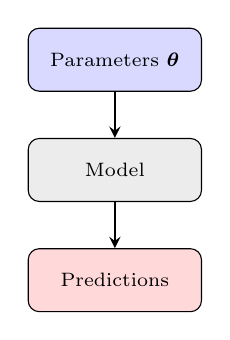
\begin{tikzpicture}
				\node[pipelinebox=blue!15, minimum width=2.2cm, font=\scriptsize] (p) at (0,0) {Parameters $\boldsymbol{\theta}$};
				\node[pipelinebox=gray!15, minimum width=2.2cm, font=\scriptsize] (m) at (0,-1.4) {Model};
				\node[pipelinebox=red!15, minimum width=2.2cm, font=\scriptsize] (d) at (0,-2.8) {Predictions};
				\draw[pipelinearr] (p) -- (m);
				\draw[pipelinearr] (m) -- (d);
			\end{tikzpicture}
		\end{column}
		\begin{column}{0.2257\textwidth}
			\centering
			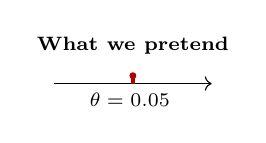
\begin{tikzpicture}[scale=0.50]
				\node[font=\scriptsize\bfseries, anchor=south] at (2,0.9) {What we pretend};
				\draw[->] (0,0.4) -- (4,0.4);
				\draw[very thick, red!70!black] (2,0.4) -- (2,0.6);
				\fill[red!70!black] (2,0.6) circle (2.5pt);
				\node[font=\scriptsize] at (2,0.0) {$\theta = 0.05\;$};
			\end{tikzpicture}

			\vspace{1mm}

			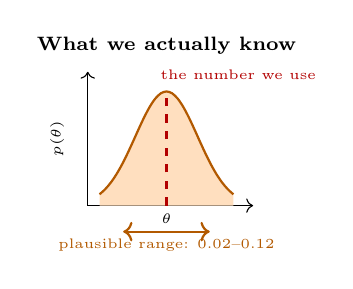
\begin{tikzpicture}[scale=0.50]
				\node[font=\scriptsize\bfseries, anchor=south] at (2,3.6) {What we actually know};
				\draw[->] (0,0) -- (4.2,0);
				\draw[->] (0,0) -- (0,3.4);
				\node[font=\tiny, rotate=90, anchor=south] at (-0.35,1.7) {$p(\theta)$};
				\fill[orange!25] plot[smooth, domain=0.3:3.7] (\x, {2.9*exp(-0.8*(\x-2)^2)}) -- (3.7,0) -- (0.3,0) -- cycle;
				\draw[thick, orange!70!black] plot[smooth, domain=0.3:3.7] (\x, {2.9*exp(-0.8*(\x-2)^2)});
				\draw[dashed, thick, red!70!black] (2,0) -- (2,2.9);
				\node[font=\tiny, red!70!black, anchor=south west] at (1.6,2.95) {the number we use};
				\node[font=\tiny] at (2,-0.32) {$\theta$};
				\draw[<->, thick, orange!70!black] (0.9,-0.66) -- (3.1,-0.66);
				\node[font=\tiny, orange!70!black] at (2,-1.0) {plausible range: 0.02--0.12};
			\end{tikzpicture}
		\end{column}
		\begin{column}{0.4518\textwidth}
			\centering
			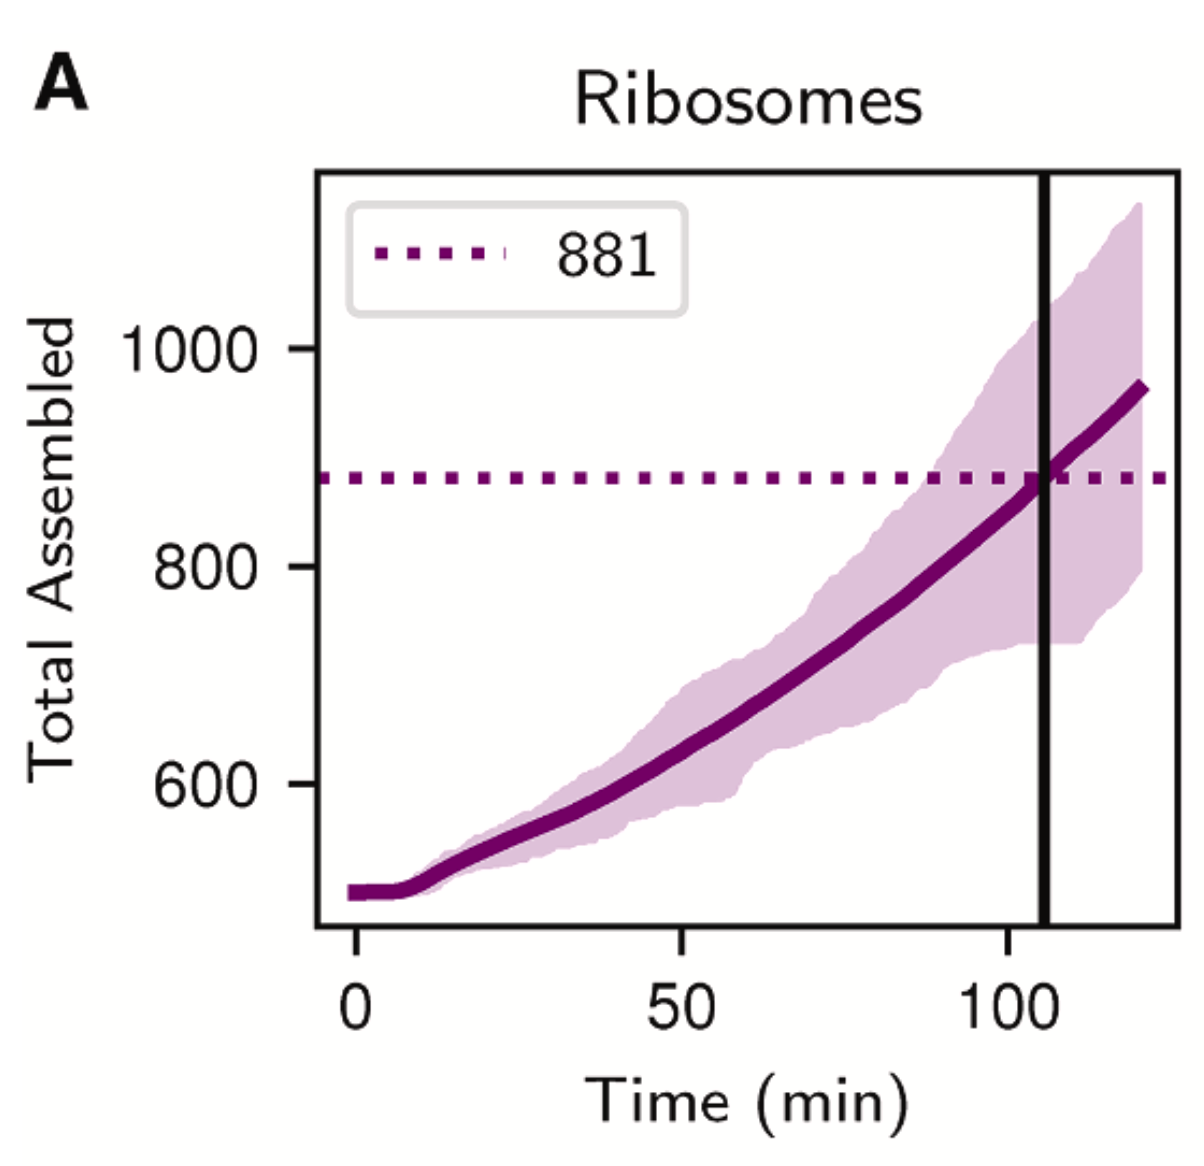
\includegraphics[height=3.6cm]{figures/ribosomes_plot.png}\\[2pt]
			{\tiny\itshape Thornburg et al., \textit{Cell} 2026, Fig.~5}
		\end{column}
	\end{columns}
	% Dividers, absolutely placed at the midpoints of the two gaps (measured from
	% the rendered page) so they do not disturb the tuned column widths.
	\begin{tikzpicture}[remember picture, overlay]
		\foreach \x in {5.00, 9.45}{
			\draw[gray!35, line width=0.4pt]
				([xshift=\x cm, yshift=-3.90cm]current page.north west) --
				([xshift=\x cm, yshift=-7.65cm]current page.north west);
		}
	\end{tikzpicture}%
\end{frame}

% ----------------------------------------------------------------
% ALTERNATIVE rendering of the toy example: trajectory fan instead of the
% flowchart above. Both are live so they can be compared; delete one.
%
% Curves are the exact solution  mRNA(t) = (k/g)(1 - e^{-g t}),  with k and g
% sampled log-uniformly across the literature ranges (k: 0.02--0.12 s^-1, a
% factor of 6; g: 0.001--0.004 s^-1, a factor of 4). Everything is expressed
% per minute (k: 1.2--7.2, g: 0.06--0.24) to keep pgfmath away from its
% small-number precision limits. The envelope is exact rather than sampled:
% (1-e^{-gt})/g decreases in g, so the extremes sit at (k_max,g_min) = 120 and
% (k_min,g_max) = 5.
\begin{frame}{But the Uncertainty Compounds}
	\small
	A minimal model with two free parameters (highlighted):
	\par\smallskip
	\centerline{$\dfrac{d[\mathrm{mRNA}]}{dt}
		= \freeparam{k_{tx}} - \freeparam{\gamma}\,[\mathrm{mRNA}]
		\qquad\Longrightarrow\qquad
		[\mathrm{mRNA}]_{ss} = \freeparam{k_{tx}}\big/\freeparam{\gamma}$}
	\par\normalsize

	\vspace{1.5mm}
	\begin{columns}[c,onlytextwidth]
	\begin{column}{0.27\textwidth}
		\centering
		\begin{tikzpicture}[
			box/.style={draw, thick, rounded corners=4pt, minimum height=0.7cm,
				minimum width=3.4cm, align=center, font=\scriptsize},
		]
			\node[box, fill=blue!12] (ktx) at (0,0)
				{$\freeparam{k_{tx}} = 0.05\;\mathrm{s}^{-1}$\\[-2pt]\tiny measured in \textit{E.\,coli}, applied to syn3A\\[-1pt]\tiny \textbf{range: 0.02--0.12}};
			\node[box, fill=blue!12, below=3mm of ktx] (gam)
				{$\freeparam{\gamma} = 0.002\;\mathrm{s}^{-1}$\\[-2pt]\tiny extrapolated from \textit{M.\,pneumoniae}\\[-1pt]\tiny \textbf{range: 0.001--0.004}};
		\end{tikzpicture}
	\end{column}
	\begin{column}{0.71\textwidth}
	\centering
	\pgfmathsetseed{20260812}
	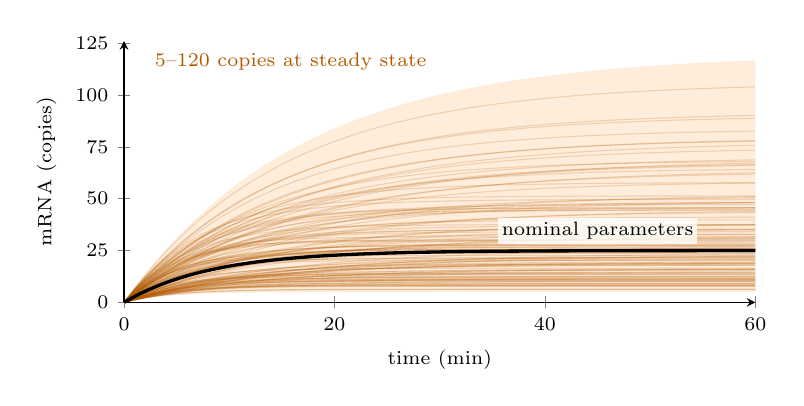
\begin{tikzpicture}
		\begin{axis}[
			width=9.6cm, height=4.9cm,
			axis lines=left,
			xlabel={time (min)},
			ylabel={mRNA (copies)},
			xmin=0, xmax=60, ymin=0, ymax=126,
			xtick={0,20,40,60},
			ytick={0,25,50,75,100,125},
			tick label style={font=\scriptsize},
			label style={font=\scriptsize},
			no markers, clip=false, axis on top,
		]
			% Exact envelope, shaded: everything the two ranges permit.
			\addplot[name path=hi, draw=none, domain=0:60, samples=80]
				{120*(1-exp(-0.06*x))};
			\addplot[name path=lo, draw=none, domain=0:60, samples=80]
				{5*(1-exp(-0.24*x))};
			\addplot[orange!14] fill between[of=hi and lo];
			% Sampled trajectories. Low opacity so overlap density reads as
			% where the plausible predictions actually concentrate -- the top of
			% the envelope needs k_max and g_min at once, so it stays empty.
			\foreach \i in {1,...,120}{
				\pgfmathsetmacro{\ku}{rnd}
				\pgfmathsetmacro{\gv}{rnd}
				\pgfmathsetmacro{\kk}{1.2*pow(6,\ku)}
				\pgfmathsetmacro{\gg}{0.06*pow(4,\gv)}
				\pgfmathsetmacro{\ss}{\kk/\gg}
				\edef\fanplot{\noexpand\addplot[thin, colSimLine, opacity=0.20,
					domain=0:60, samples=60] {\ss*(1-exp(-\gg*x))};}
				\fanplot
			}
			% The single trajectory a forward simulator would report
			\addplot[very thick, black, domain=0:60, samples=80]
				{25*(1-exp(-0.12*x))};
			\node[anchor=south, font=\scriptsize, fill=white, fill opacity=0.8,
				text opacity=1, inner sep=1.5pt] at (axis cs:45,28)
				{nominal parameters};
			% Range called out inside the axis: the upper-left is empty because
			% the envelope climbs slowly, so it costs no horizontal width.
			\node[anchor=north west, font=\scriptsize, colSimLine, align=left]
				at (axis cs:2,125) {5--120 copies at steady state\\[-1pt]
				{}};
		\end{axis}
	\end{tikzpicture}
	\end{column}
	\end{columns}

\end{frame}

% VERBAL: When MC4D predicts a 110-minute doubling time, we cannot distinguish
% whether (a) the prediction is robust across plausible parameters, or
% (b) it is fragile and depends on specific choices.




% ----------------------------------------------------------------
% The assembly pipeline, drawn so that it looks as lossy as it is: the
% point-estimate boxes are ghost-plus-spike glyphs (the fitted width is drawn,
% then shown being dropped), and the coupling that isolated fitting never sees
% is crossed out between the fit boxes.
\begin{frame}{No information/uncertainty flows between modules}
	\small
	Subsystems are calibrated in isolation, then assembled from point estimates.
	\par\normalsize

	\vspace{0.5mm}
	\centering
	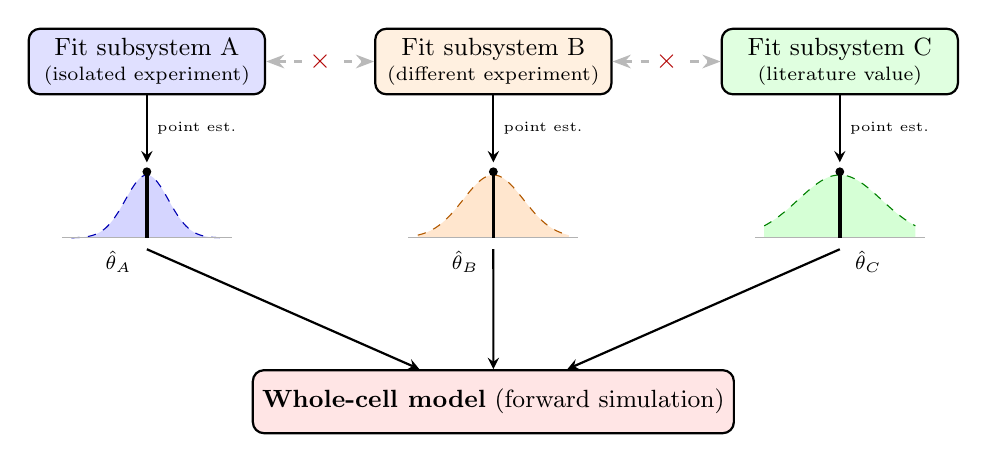
\begin{tikzpicture}[
		scale=0.80,
		wfbox/.style={draw, thick, rounded corners=4pt, minimum height=0.8cm,
			minimum width=3cm, align=center, font=\small},
		>=Stealth
	]
		\node[wfbox, fill=blue!12]   (fitA) at (0,3.6)  {Fit subsystem A\\[-2pt]\scriptsize (isolated experiment)};
		\node[wfbox, fill=orange!12] (fitB) at (5.5,3.6) {Fit subsystem B\\[-2pt]\scriptsize (different experiment)};
		\node[wfbox, fill=green!12]  (fitC) at (11,3.6) {Fit subsystem C\\[-2pt]\scriptsize (literature value)};

		% The coupling that fitting in isolation never sees
		\draw[<->, thick, gray!55, dashed] (fitA.east) -- (fitB.west);
		\draw[<->, thick, gray!55, dashed] (fitB.east) -- (fitC.west);
		\node[circle, fill=white, inner sep=0.5pt, text=colWarnLine,
			font=\bfseries] at ($(fitA.east)!0.5!(fitB.west)$) {$\times$};
		\node[circle, fill=white, inner sep=0.5pt, text=colWarnLine,
			font=\bfseries] at ($(fitB.east)!0.5!(fitC.west)$) {$\times$};

		% Point estimates, drawn as the collapse they are.
		% \lx puts the label on the side of the spike its own assembly arrow does
		% not leave from: A's arrow departs rightward and B's straight down, so
		% both labels sit left; C's angles back in towards the box at x=5.5 and
		% would bisect a left-hand label, so C mirrors.
		\foreach \cx/\sd/\cfill/\cline/\lbl/\lx in {%
			0/0.34/blue!30/blue!70!black/A/-0.45,
			5.5/0.48/orange!35/orange!70!black/B/-0.45,
			11/0.66/green!30/green!50!black/C/0.45}
		{
			\begin{scope}[shift={(\cx,0.8)}]
				\fill[\cfill, opacity=0.55]
					plot[smooth, domain=-1.2:1.2, samples=36]
					(\x, {1.0*exp(-0.5*(\x/\sd)^2)}) -- (1.2,0) -- (-1.2,0) -- cycle;
				\draw[thin, dashed, \cline]
					plot[smooth, domain=-1.2:1.2, samples=36]
					(\x, {1.0*exp(-0.5*(\x/\sd)^2)});
				\draw[thin, gray!60] (-1.35,0) -- (1.35,0);
				\draw[line width=1.3pt, black] (0,0) -- (0,1.05);
				\fill[black] (0,1.05) circle (0.07);
				% anchor=north, not north east: the label is centred on \lx so the
				% left- and right-hand placements are mirror images of each other.
				\node[font=\scriptsize, anchor=north] at (\lx,-0.05)
					{$\hat\theta_\lbl$};
			\end{scope}
			\draw[pipelinearr] (\cx,3.1) -- (\cx,2.0)
				node[midway, right, font=\tiny] {point est.};
		}

		\node[wfbox, fill=red!10, minimum width=5cm] (wcm) at (5.5,-1.8)
			{\textbf{Whole-cell model} (forward simulation)};

		% Drawn after the box so TikZ can clip each arrow to its border; the
		% outer columns lie outside the box footprint, so they angle inward.
		\draw[pipelinearr] (0,0.62)   -- (wcm);
		\draw[pipelinearr] (5.5,0.62) -- (wcm);
		\draw[pipelinearr] (11,0.62)  -- (wcm);
	\end{tikzpicture}

	\vspace{1mm}
	\alert{\small Uncertainty is computed, then discarded; the coupling
	($\boldsymbol{\times}$) is never seen at all.}
\end{frame}

% ----------------------------------------------------------------
%\begin{frame}{Why Not Just Run It a Thousand Times?}
%	\small
%	A natural response: \emph{perturb the parameters, run an ensemble, get a distribution of predictions.} Two reasons this doesn't close the gap:
%
%	\medskip
%	\begin{columns}[T]
%		\begin{column}{0.48\textwidth}
%			\textbf{1. Ensemble $\neq$ posterior.}
%
%			\smallskip
%			Without a likelihood, you cannot:
%			\begin{itemize}\itemsep1pt
%				\item Condition on observed data
%				\item Weight parameter combinations by plausibility
%				\item Compare models or update beliefs
%				\item Compute identifiability, BOED, Bayes factors
%			\end{itemize}
%
%			\smallskip
%			{\scriptsize A spread of point predictions is not a probability distribution.}
%		\end{column}
%		\begin{column}{0.48\textwidth}
%			\textbf{2. Each run is expensive.}
%
%			\smallskip
%			MC4D: ${\sim}$300 GPU-hours per replicate.\\
%			A 1000-run ensemble: $3 \times 10^5$ GPU-hours.
%
%			\smallskip
%			Even if you had a likelihood, the architecture cannot evaluate it efficiently:
%			\begin{itemize}\itemsep1pt
%				\item No gradient path $\to$ no HMC, no AD
%				\item IO at every module boundary
%				\item No surrogate-friendly substrate
%			\end{itemize}
%		\end{column}
%	\end{columns}
%
%	\vfill
%	\centering
%	\alert{Two architectural gaps: \textbf{probability} and \textbf{substrate}.}
%\end{frame}


% ================================================================
% SECTION 2: InferCell
% ================================================================
\section{InferCell}


% ----------------------------------------------------------------
\begin{frame}{Inverting the Question}
	\begin{columns}[T]
		\begin{column}{0.48\textwidth}
			\centering
			\textbf{Forward simulation}\\[6pt]
			% Coordinates in cm and no scale= key: TikZ scales positions but not
			% node minimum heights, so under the old scale=0.75 the 1.2cm pitch
			% became 0.9cm against 0.8cm-tall boxes and left 1mm of arrow. A 1.5cm
			% pitch gives 7mm. Same geometry in the inference column opposite and
			% on the Summary slide, so all three read as one object.
			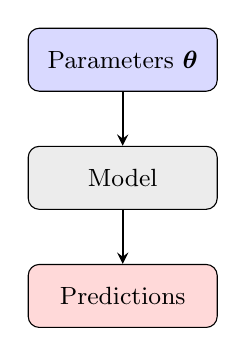
\begin{tikzpicture}
				\node[pipelinebox=blue!15, minimum width=2.4cm] (p) at (0,0) {Parameters $\boldsymbol{\theta}$};
				\node[pipelinebox=gray!15, minimum width=2.4cm] (m) at (0,-1.5) {Model};
				\node[pipelinebox=red!15, minimum width=2.4cm] (d) at (0,-3.0) {Predictions};
				\draw[pipelinearr] (p) -- (m);
				\draw[pipelinearr] (m) -- (d);
			\end{tikzpicture}\\[4pt]
			{\small \textit{``Given $\theta$, what does the cell do?''}}
		\end{column}
		\begin{column}{0.48\textwidth}
			\centering
			\textbf{Inference}\\[6pt]
			% Same geometry as the forward diagram opposite --- see the comment
			% there. Repeated verbatim on the Summary slide.
			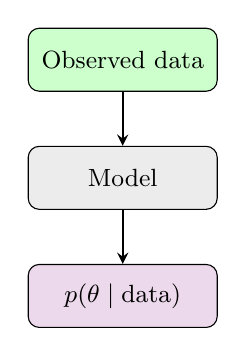
\begin{tikzpicture}
				\node[pipelinebox=green!20, minimum width=2.4cm] (d) at (0,0) {Observed data};
				\node[pipelinebox=gray!15, minimum width=2.4cm] (m) at (0,-1.5) {Model};
				\node[pipelinebox=colPost, minimum width=2.4cm] (p) at (0,-3.0) {$p(\theta \mid \text{data})$};
				\draw[pipelinearr] (d) -- (m);
				\draw[pipelinearr] (m) -- (p);
			\end{tikzpicture}\\[4pt]
			{\small \textit{``Given data, what $\theta$ are consistent?''}}
		\end{column}
	\end{columns}
\end{frame}




% SPEAKER NOTES:
% - The gap is semantic: the architecture has no representation for
%   probability. You cannot bolt a likelihood onto a system that stores
%   parameters as floats without rewriting the data structures.
% - Adding ABC on top of MC4D doesn't fix this: you can sample, but the
%   model itself still has no probabilistic semantics. Module boundaries
%   carry no distribution -- only point values.
% - InferCell makes parameters distributions natively, so every module
%   boundary can carry uncertainty by construction.
% - This slide is the first gap: probability. The next slide is the second:
%   substrate. Both are answered together on the design-principles slide.
%   Do not preview the polyglot argument here -- it lands harder as the
%   answer to "why hasn't anyone done this?" than as another complaint.


% ----------------------------------------------------------------
% The feasibility gap, placed straight after the pivot so it answers the
% question the audience is already asking. It also exists to earn "one
% language, one computational graph" two slides later: without a picture of
% the polyglot stack first, that bullet reads as a language preference
% rather than a requirement. Diagram promoted from the old backup
% "Why Pure Julia?" slide, reframed as an obstacle rather than an answer.
\begin{frame}{And another thing! - WCMs are polyglot stacks}
	\small
SOTA 4DMC = four solvers in three languages, glued by a Python script.
	\par\normalsize

	\vspace{1mm}
	\begin{columns}[c,onlytextwidth]
		\begin{column}{0.55\textwidth}
			% \small, not \scriptsize: with each gloss cut to a phrase every item
			% sets in one line at this column width, so the column no longer has
			% to buy space with type size. The detail that was here is spoken --
			% see speaker-notes.md. itemsep up from 3pt to fill the freed height.
			\small
			\begin{itemize}\itemsep6pt
				\item \textbf{HPC penalties} --- serialise, spawn, copy at every
				boundary.

				\item \textbf{No differentiability} --- AD dies at the
				boundary.

				\item \textbf{No composability} --- every swap is cross-language
				plumbing.

				\item \textbf{No hybrid inference} --- NUTS and SBI, separate
				ecosystems.

				\item \textbf{Engineering friction} --- many toolchains, broken
				stack traces.
			\end{itemize}
		\end{column}
		\begin{column}{0.43\textwidth}
			\centering
			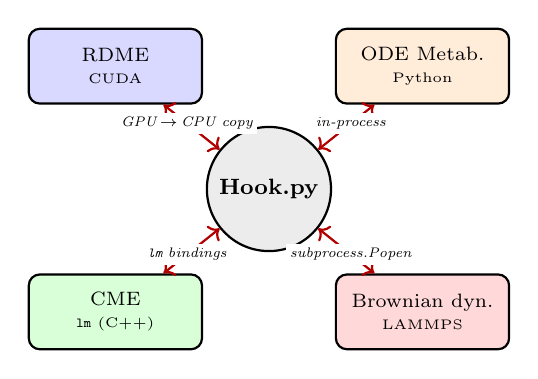
\begin{tikzpicture}[
				scale=0.52,
				every node/.style={font=\scriptsize},
				iolabel/.style={font=\tiny\itshape, black, fill=white, inner sep=1.5pt}
			]
				\node[draw, rounded corners=4pt, thick, fill=blue!15,
				      minimum height=0.95cm, minimum width=2.2cm, align=center]
				     (rdme) at (-2,5) {RDME\\\tiny CUDA};
				\node[draw, rounded corners=4pt, thick, fill=orange!15,
				      minimum height=0.95cm, minimum width=2.2cm, align=center]
				     (ode) at (5.5,5) {ODE Metab.\\\tiny Python};
				\node[draw, rounded corners=4pt, thick, fill=green!15,
				      minimum height=0.95cm, minimum width=2.2cm, align=center]
				     (cme) at (-2,-1) {CME\\\tiny \texttt{lm} (C++)};
				\node[draw, rounded corners=4pt, thick, fill=red!15,
				      minimum height=0.95cm, minimum width=2.2cm, align=center]
				     (bd) at (5.5,-1) {Brownian dyn.\\\tiny LAMMPS};
				\node[draw, circle, thick, fill=gray!15, minimum size=1.1cm, align=center]
				     (sim) at (1.75,2) {\textbf{\footnotesize Hook.py}};
				\draw[<->, thick, colWarnLine] (rdme) -- node[iolabel, pos=0.42]
				     {GPU\,$\to$\,CPU copy} (sim);
				\draw[<->, thick, colWarnLine] (ode) -- node[iolabel, pos=0.42]
				     {in-process} (sim);
				\draw[<->, thick, colWarnLine] (cme) -- node[iolabel, pos=0.42]
				     {\texttt{lm} bindings} (sim);
				\draw[<->, thick, colWarnLine] (bd) -- node[iolabel, pos=0.42]
				     {subprocess.Popen} (sim);
			\end{tikzpicture}
		\end{column}
	\end{columns}

\end{frame}

% VERBAL: the previous slide said the architecture never asks the inference
% question. This one says that even if it wanted to, the runtime could not
% answer it -- a gradient does not survive subprocess.Popen. Hand straight
% off to the design principles: that is what the single stack buys.



% ----------------------------------------------------------------
%\begin{frame}{What Inference Enables}
%
%	Inference lets you ask scientific questions that forward simulation cannot pose.
%
%	\bigskip
%	\begin{columns}[T]
%		\begin{column}{0.58\textwidth}
%			\begin{enumerate}\itemsep8pt
%				\item \textbf{Know which predictions to trust.}\\
%				{\small UQ. Probabilistic prediction. \\ \textit{"Is this prediction robust, or does it depend on parameter choices we're not confident about?"} }
%
%				\item \textbf{Learn biology from data.}\\
%				{\small Which parameters are identifiable? Does the modelling formalism matter (ODE vs SSA)? What should we measure next?}
%
%				\item \textbf{Discover when your model is wrong.}\\
%				{\small Posteriors far from literature values, or formalisms that disagree $\implies$ misspecification}
%			\end{enumerate}
%		\end{column}
%		\begin{column}{0.38\textwidth}
%			\centering
%			% 1. Predictions with uncertainty
%			\begin{tikzpicture}[scale=0.55]
%				\draw[->] (0,0) -- (4.2,0) node[right, font=\scriptsize] {$t$};
%				\draw[->] (0,0) -- (0,2.6);
%				\fill[violet!12] plot[smooth, domain=0:4] (\x, {1.8*(1-exp(-0.7*\x)) + 0.4})
%					-- plot[smooth, domain=4:0] (\x, {1.8*(1-exp(-0.7*\x)) - 0.4}) -- cycle;
%				\draw[thin, violet!40] plot[smooth, domain=0:4] (\x, {1.9*(1-exp(-0.65*\x)) + 0.15});
%				\draw[thin, violet!40] plot[smooth, domain=0:4] (\x, {1.7*(1-exp(-0.75*\x)) - 0.1});
%				\draw[thick, colPostLine] plot[smooth, domain=0:4] (\x, {1.8*(1-exp(-0.7*\x))});
%				\node[font=\scriptsize, colPostLine, anchor=west] at (2.5,2.3) {95\% CI};
%			\end{tikzpicture}
%
%			\vspace{6pt}
%
%			% 2. Identifiability: posterior vs prior
%			\begin{tikzpicture}[scale=0.55]
%				\draw[->] (0,0) -- (4,0) node[right, font=\scriptsize] {$\theta$};
%				\draw[->] (0,0) -- (0,2.4);
%				% Broad prior
%				\fill[gray!10] plot[smooth, domain=0.2:3.8] (\x, {0.7*exp(-0.2*(\x-2)^2)}) -- (3.8,0) -- (0.2,0) -- cycle;
%				\draw[thick, gray!50] plot[smooth, domain=0.2:3.8] (\x, {0.7*exp(-0.2*(\x-2)^2)});
%				% Tight posterior
%				\fill[colPost] plot[smooth, domain=0.3:3.7] (\x, {2.2*exp(-1.5*(\x-2.1)^2)}) -- (3.7,0) -- (0.3,0) -- cycle;
%				\draw[thick, colPostLine] plot[smooth, domain=0.3:3.7] (\x, {2.2*exp(-1.5*(\x-2.1)^2)});
%				\node[font=\scriptsize, gray!60, anchor=west] at (3.5,0.8) {prior};
%				\node[font=\scriptsize, colPostLine, anchor=west] at (3.5,1.8) {posterior};
%			\end{tikzpicture}
%
%			\vspace{6pt}
%
%			% 3. Model criticism: two formalisms disagree
%			\begin{tikzpicture}[scale=0.55]
%				\draw[->] (0,0) -- (4.2,0) node[right, font=\scriptsize] {$\theta$};
%				\draw[->] (0,0) -- (0,2.2);
%				\fill[blue!10] plot[smooth, domain=0.3:3.2] (\x, {1.8*exp(-1.8*(\x-1.4)^2)}) -- (3.2,0) -- (0.3,0) -- cycle;
%				\draw[thick, colODELine] plot[smooth, domain=0.3:3.2] (\x, {1.8*exp(-1.8*(\x-1.4)^2)});
%				\fill[orange!10] plot[smooth, domain=1.0:4.0] (\x, {1.6*exp(-1.5*(\x-2.8)^2)}) -- (4.0,0) -- (1.0,0) -- cycle;
%				\draw[thick, colSimLine] plot[smooth, domain=1.0:4.0] (\x, {1.6*exp(-1.5*(\x-2.8)^2)});
%				\node[font=\scriptsize, colODELine] at (0.7,1.9) {ODE};
%				\node[font=\scriptsize, colSimLine] at (3.6,1.7) {SSA};
%				\node[font=\scriptsize\itshape, colWarnLine, anchor=north] at (2.1,-0.3) {disagree $\Rightarrow$ formalism matters};
%			\end{tikzpicture}
%		\end{column}
%	\end{columns}
%\end{frame}
%


%\begin{frame}{What Inference Enables}
%	
%	Inference lets you ask scientific questions that forward simulation cannot pose.
%	
%	\bigskip
%	\begin{columns}[T]
%		\begin{column}{0.58\textwidth}
%			\begin{enumerate}\itemsep8pt
%				\item \textbf{Know which predictions to trust.}\\
%				{\small UQ. \textit{"Is this prediction robust, or does it depend on parameter choices we're not confident about?"} }
%				\item \textbf{Learn biology from data.}\\
%				{\small Identifiability, model selection, Bayesian OED. \\ \textit{``What can we actually learn from the data we have, and what should we measure next?"}}
%				\item \textbf{Discover when your model is wrong.}\\
%				{\small Posteriors far from literature values, or formalisms that disagree $\implies$ misspecification \\ \textit{"Where does our model break down?"} }
%			\end{enumerate}
%		\end{column}
%		\begin{column}{0.38\textwidth}
%			\centering
%			% 1. Predictions with uncertainty
%			\begin{tikzpicture}[scale=0.55]
%				\draw[->] (0,0) -- (4.2,0) node[right, font=\scriptsize] {$t$};
%				\draw[->] (0,0) -- (0,2.6);
%				\fill[violet!12] plot[smooth, domain=0:4] (\x, {1.8*(1-exp(-0.7*\x)) + 0.4})
%				-- plot[smooth, domain=4:0] (\x, {1.8*(1-exp(-0.7*\x)) - 0.4}) -- cycle;
%				\draw[thin, violet!40] plot[smooth, domain=0:4] (\x, {1.9*(1-exp(-0.65*\x)) + 0.15});
%				\draw[thin, violet!40] plot[smooth, domain=0:4] (\x, {1.7*(1-exp(-0.75*\x)) - 0.1});
%				\draw[thick, colPostLine] plot[smooth, domain=0:4] (\x, {1.8*(1-exp(-0.7*\x))});
%				\node[font=\scriptsize, colPostLine, anchor=west] at (2.5,2.3) {95\% CI};
%			\end{tikzpicture}
%			
%			\vspace{6pt}
%			
%			% 2. Identifiability: posterior vs prior
%			\begin{tikzpicture}[scale=0.55]
%				\draw[->] (0,0) -- (4,0) node[right, font=\scriptsize] {$\theta$};
%				\draw[->] (0,0) -- (0,2.4);
%				% Broad prior
%				\fill[gray!10] plot[smooth, domain=0.2:3.8] (\x, {0.7*exp(-0.2*(\x-2)^2)}) -- (3.8,0) -- (0.2,0) -- cycle;
%				\draw[thick, gray!50] plot[smooth, domain=0.2:3.8] (\x, {0.7*exp(-0.2*(\x-2)^2)});
%				% Tight posterior
%				\fill[colPost] plot[smooth, domain=0.3:3.7] (\x, {2.2*exp(-1.5*(\x-2.1)^2)}) -- (3.7,0) -- (0.3,0) -- cycle;
%				\draw[thick, colPostLine] plot[smooth, domain=0.3:3.7] (\x, {2.2*exp(-1.5*(\x-2.1)^2)});
%				\node[font=\scriptsize, gray!60, anchor=west] at (3.5,0.8) {prior};
%				\node[font=\scriptsize, colPostLine, anchor=west] at (3.5,1.8) {posterior};
%			\end{tikzpicture}
%			
%			\vspace{6pt}
%			
%			% 3. Model criticism: two formalisms disagree
%			\begin{tikzpicture}[scale=0.55]
%				\draw[->] (0,0) -- (4.2,0) node[right, font=\scriptsize] {$\theta$};
%				\draw[->] (0,0) -- (0,2.2);
%				\fill[blue!10] plot[smooth, domain=0.3:3.2] (\x, {1.8*exp(-1.8*(\x-1.4)^2)}) -- (3.2,0) -- (0.3,0) -- cycle;
%				\draw[thick, colODELine] plot[smooth, domain=0.3:3.2] (\x, {1.8*exp(-1.8*(\x-1.4)^2)});
%				\fill[orange!10] plot[smooth, domain=1.0:4.0] (\x, {1.6*exp(-1.5*(\x-2.8)^2)}) -- (4.0,0) -- (1.0,0) -- cycle;
%				\draw[thick, colSimLine] plot[smooth, domain=1.0:4.0] (\x, {1.6*exp(-1.5*(\x-2.8)^2)});
%				\node[font=\scriptsize, colODELine] at (0.7,1.9) {ODE};
%				\node[font=\scriptsize, colSimLine] at (3.6,1.7) {SSA};
%				\node[font=\scriptsize\itshape, colWarnLine, anchor=north] at (2.1,-0.3) {disagree $\Rightarrow$ formalism matters};
%			\end{tikzpicture}
%		\end{column}
%	\end{columns}
%\end{frame}




% ================================================================
% SECTION 3: Architecture
% ================================================================
\section{Architecture}


% ----------------------------------------------------------------
% The reveal. Deliberately an OVERVIEW, not a payoff slide: "What Becomes
% Possible" is next and owns the payoff, so listing capabilities here would
% pay twice for the same ground. Banner names the thing, three bullets say
% what it is, figure shows how it is built.
% The figure is a zoom composition rather than another pipeline diagram --
% the pipeline shape already appeared on slide 5, so it would re-render a
% known idea instead of adding the new one. The old coupled-model pipeline
% figure survives on the "Conditioning the Whole Model" backup.
\begin{frame}{InferCell}
	\vspace{-1mm}
	% Link here because it belongs where the thing is named. Own line rather than
	% flush right -- \hfill is a no-op once the sentence above fills its line, so
	% the break is explicit instead.
	% (This used to add "and the closing slide now ends on the four asks with
	% nothing competing for attention". That four-asks slide is gone and the
	% Summary slide repeats the link deliberately: it is the last thing on screen
	% during discussion, and remote attendees screenshot it.)
	InferCell is a composable, inference-first whole-cell modelling framework in
	Julia.\\
	{\scriptsize\href{https://github.com/MACSYS-CoE/InferCell}{github.com/MACSYS-CoE/InferCell}}
%	\begin{center}
%		\colorbox{oxfordblue}{\parbox{0.965\textwidth}{\centering\color{white}\small
%		}}
%	\end{center}

	\vspace{0.5mm}
	\begin{columns}[c,onlytextwidth]
		\begin{column}{0.53\textwidth}
			\small
			\begin{itemize}\itemsep3pt
				\item \textbf{Inference-first}\\
				{\scriptsize UQ  \& probabilistic prediction is is built in. Parameters are distributions natively. Boundaries carry posteriors}

				\item \textbf{Modular.}\\
				{\scriptsize Swap ODE for SSA, or a solver for an ML surrogate.
				The inference layer is unchanged.}

				\item \textbf{Pure Julia.}\\
				{\scriptsize One language, one computational graph. }
			\end{itemize}
		\end{column}
		\begin{column}{0.45\textwidth}
			\centering
			% Zoom composition: the whole stack as one graph (overview), with a
			% magnified callout on one module seam (mechanism). Modules sit at
			% the BOTTOM of the stack so the zoom lines drop straight into the
			% callout without crossing the diagram. All coordinates in cm and no
			% scale= key: TikZ scales positions but not node minimum widths, so
			% mixing the two makes a tiled layer come apart.
			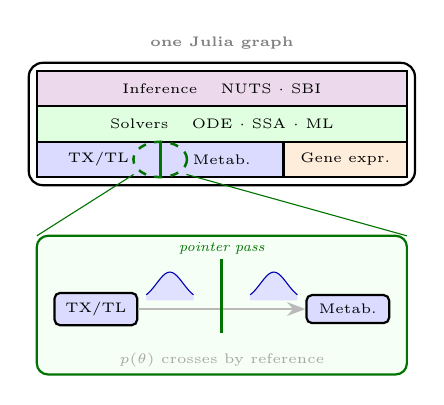
\begin{tikzpicture}[
				lay/.style={draw, thick, minimum width=4.7cm,
					minimum height=0.45cm, font=\tiny, align=center},
				seg/.style={draw, thick, minimum width=1.5667cm,
					minimum height=0.45cm, font=\tiny, align=center},
				cbox/.style={draw, thick, rounded corners=2pt, minimum width=1.05cm,
					minimum height=0.34cm, font=\tiny, align=center},
				>=Stealth
			]
			% ===== Overview: the single graph =====
			\node[lay, fill=colPost]   (inf) at (0,3.15) {Inference \;\; NUTS $\cdot$ SBI};
			\node[lay, fill=green!12]  (sol) at (0,2.70) {Solvers \;\; ODE $\cdot$ SSA $\cdot$ ML};
			\node[seg, fill=blue!14]   (m1)  at (-1.5667,2.25) {TX/TL};
			\node[seg, fill=blue!14]   (m2)  at (0,2.25)       {Metab.};
			\node[seg, fill=orange!14] (m3)  at (1.5667,2.25)  {Gene expr.};

			\node[draw, thick, rounded corners=5pt, fit=(inf)(sol)(m1)(m3),
				inner sep=2.5pt] (graph) {};
			\node[font=\tiny\bfseries, text=gray, anchor=south]
				at ([yshift=1pt]graph.north) {one Julia graph};

			% The seam itself, then a magnifier ring around it
			\draw[line width=1.1pt, green!45!black] (-0.783,2.035) -- (-0.783,2.465);
			% Ellipse, not a circle: a circle wide enough to read as a lens
			% would poke up into the Solvers layer and cut its label.
			\draw[dashed, line width=0.9pt, green!45!black]
				(-0.783,2.25) ellipse (0.34 and 0.225);

			% ===== Zoom lines into the callout =====
			\draw[thin, green!45!black] (-1.12,2.06) -- (-2.35,1.28);
			\draw[thin, green!45!black] (-0.45,2.06) -- (2.35,1.28);

			% ===== Callout: what the seam actually is =====
			\draw[thick, rounded corners=4pt, green!45!black, fill=green!4]
				(-2.35,-0.48) rectangle (2.35,1.28);
			\node[cbox, fill=blue!14]   (ca) at (-1.6,0.35) {TX/TL};
			\node[cbox, fill=blue!14]   (cb) at (1.6,0.35)  {Metab.};
			\draw[->, thick, gray!55] (ca) -- (cb);
			\draw[line width=1.1pt, green!45!black] (0,0.05) -- (0,0.98);
			\node[font=\tiny\itshape, text=green!45!black] at (0,1.12) {pointer pass};
			\begin{scope}[shift={(-0.66,0.46)}]
				\fill[colODE] plot[smooth, domain=-0.3:0.3, samples=21]
					(\x,{0.36*exp(-18*\x*\x)}) -- (0.3,0) -- (-0.3,0) -- cycle;
				\draw[thin, colODELine] plot[smooth, domain=-0.3:0.3, samples=21]
					(\x,{0.36*exp(-18*\x*\x)});
			\end{scope}
			\begin{scope}[shift={(0.66,0.46)}]
				\fill[colODE] plot[smooth, domain=-0.3:0.3, samples=21]
					(\x,{0.36*exp(-18*\x*\x)}) -- (0.3,0) -- (-0.3,0) -- cycle;
				\draw[thin, colODELine] plot[smooth, domain=-0.3:0.3, samples=21]
					(\x,{0.36*exp(-18*\x*\x)});
			\end{scope}
			\node[font=\tiny, text=gray!70] at (0,-0.30)
				{$p(\theta)$ crosses by reference};
			\end{tikzpicture}\\[3pt]
		\end{column}
	\end{columns}
\end{frame}

% VERBAL:
% - Bridge in from the previous slide, which ended on "not computable here":
%   "so we built the substrate where it is." Without a bridge this slide
%   opens cold on a definition.
% - The design test at every module boundary is one question: "how does
%   inference cross this?" That test is what produced all three bullets.
%   (Was a bullet of its own; describes our process, not the audience's
%   payoff, so it is better said than shown.)
% - Do not list capabilities here. "What Becomes Possible" is next.


%% ----------------------------------------------------------------
%\begin{frame}{What Becomes Possible}
%	\scriptsize
%	Scientific questions that forward simulation cannot pose:
%	
%	\medskip
%	\begin{columns}[T]
%		\begin{column}{0.48\textwidth}
%			\textbf{Quantitative biology}
%			\begin{itemize}\itemsep0pt\parskip0pt
%				\item Which parameters does the data actually constrain?
%				\item Is mechanism $X$ consistent with the observations?
%				\item Are competing hypotheses distinguishable?
%				\item Where does the model fail to reproduce reality?
%			\end{itemize}
%			
%			\medskip
%			\textbf{Structural inference}
%			\begin{itemize}\itemsep0pt\parskip0pt
%				\item Discover which reactions are present, from data
%				\item Recover dynamically-equivalent CRN families
%				\item Quantify structural uncertainty alongside parameters
%			\end{itemize}
%		\end{column}
%		\begin{column}{0.48\textwidth}
%			\textbf{Experimental design}
%			\begin{itemize}\itemsep0pt\parskip0pt
%				\item What should I measure next?
%				\item Which experiment maximises information gain?
%				\item What's the value of a new dataset before running it?
%				\item How does information propagate between subsystems?
%			\end{itemize}
%			
%			\medskip
%			\textbf{Model criticism}
%			\begin{itemize}\itemsep0pt\parskip0pt
%				\item Posterior predictive checks for misspecification
%				\item Compare formalisms (ODE vs SSA) on the same data
%				\item Detect when literature priors conflict with observations
%			\end{itemize}
%		\end{column}
%	\end{columns}
%	
%	\vfill
%	\centering
%	\alert{Forward simulation never reveals these. The framework is what makes them rigorous.}
%\end{frame}


\begin{frame}{What Becomes Possible (Science)}
	\small
	Questions that forward simulation cannot pose:
	\smallskip
	\begin{columns}[T]

		\begin{column}{0.49\textwidth}
			\begin{itemize}\itemsep3pt\parskip0pt
				\item \textbf{Probabilistic prediction}\\[1pt]
				{\scriptsize\itshape ``Is doubling time 110\,$\pm$\,5\,min, or 60--200?''}
				\item \textbf{Parameter calibration}\\[1pt]
				{\scriptsize\itshape ``What is $k_{tx}$ for this gene, given our data?''}
				\item \textbf{Identifiability}\\[1pt]
				{\scriptsize\itshape ``Does data constrain $k_{tx}$ alone, or only $k_{tx}/\gamma$?''}
			\end{itemize}
		\end{column}
		\begin{column}{0.49\textwidth}
			\begin{itemize}\itemsep3pt\parskip0pt
				\item \textbf{Model selection}\\[1pt]
				{\scriptsize\itshape ``Does the data prefer ODE or SSA dynamics?''}
				\item \textbf{Experimental design}\\[1pt]
				{\scriptsize\itshape ``Which experiment most reduces uncertainty in $\gamma_{prot}$?''}
				\item \textbf{Fundamental biology}\\[1pt]
				{\scriptsize\itshape ``Does the data require enzyme feedback in metabolism?''}
			\end{itemize}
		\end{column}
	\end{columns}

	\vfill
	\begin{columns}[b]
		\begin{column}{0.32\textwidth}
			\centering
			% 1. Predictions with uncertainty
			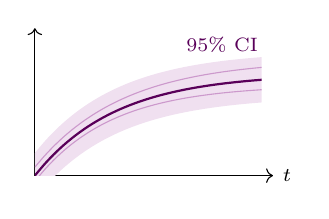
\begin{tikzpicture}[scale=0.72]
				\draw[->] (0,0) -- (4.2,0) node[right, font=\scriptsize] {$t$};
				\draw[->] (0,0) -- (0,2.6);
				\begin{scope}
					\clip (0,0) rectangle (4.2,2.6);
					\fill[violet!12] plot[smooth, domain=0:4] (\x, {1.8*(1-exp(-0.7*\x)) + 0.4})
						-- plot[smooth, domain=4:0] (\x, {1.8*(1-exp(-0.7*\x)) - 0.4}) -- cycle;
					\draw[thin, violet!40] plot[smooth, domain=0:4] (\x, {1.9*(1-exp(-0.65*\x)) + 0.15});
					\draw[thin, violet!40] plot[smooth, domain=0:4] (\x, {1.7*(1-exp(-0.75*\x)) - 0.1});
					\draw[thick, colPostLine] plot[smooth, domain=0:4] (\x, {1.8*(1-exp(-0.7*\x))});
				\end{scope}
				\node[font=\scriptsize, colPostLine, anchor=west] at (2.5,2.3) {95\% CI};
			\end{tikzpicture}
		\end{column}
		\begin{column}{0.32\textwidth}
			\centering
			% 2. Mechanistic inference: model selection
			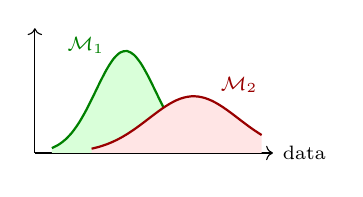
\begin{tikzpicture}[scale=0.72]
				\draw[->] (0,0) -- (4.2,0) node[right, font=\scriptsize] {data};
				\draw[->] (0,0) -- (0,2.2);
				\fill[green!15] plot[smooth, domain=0.3:3.2] (\x, {1.8*exp(-1.8*(\x-1.6)^2)}) -- (3.2,0) -- (0.3,0) -- cycle;
				\draw[thick, green!50!black] plot[smooth, domain=0.3:3.2] (\x, {1.8*exp(-1.8*(\x-1.6)^2)});
				\fill[red!10] plot[smooth, domain=1.0:4.0] (\x, {1.0*exp(-0.8*(\x-2.8)^2)}) -- (4.0,0) -- (1.0,0) -- cycle;
				\draw[thick, red!60!black] plot[smooth, domain=1.0:4.0] (\x, {1.0*exp(-0.8*(\x-2.8)^2)});
				\node[font=\scriptsize, green!50!black] at (0.9,1.9) {$\mathcal{M}_1$};
				\node[font=\scriptsize, red!60!black] at (3.6,1.2) {$\mathcal{M}_2$};
			\end{tikzpicture}
		\end{column}
		\begin{column}{0.32\textwidth}
			\centering
			% 3. Identifiability: posterior vs prior
			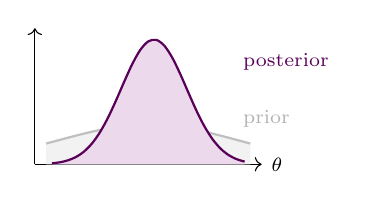
\begin{tikzpicture}[scale=0.72]
				\draw[->] (0,0) -- (4,0) node[right, font=\scriptsize] {$\theta$};
				\draw[->] (0,0) -- (0,2.4);
				\fill[gray!10] plot[smooth, domain=0.2:3.8] (\x, {0.7*exp(-0.2*(\x-2)^2)}) -- (3.8,0) -- (0.2,0) -- cycle;
				\draw[thick, gray!50] plot[smooth, domain=0.2:3.8] (\x, {0.7*exp(-0.2*(\x-2)^2)});
				\fill[colPost] plot[smooth, domain=0.3:3.7] (\x, {2.2*exp(-1.5*(\x-2.1)^2)}) -- (3.7,0) -- (0.3,0) -- cycle;
				\draw[thick, colPostLine] plot[smooth, domain=0.3:3.7] (\x, {2.2*exp(-1.5*(\x-2.1)^2)});
				\node[font=\scriptsize, gray!60, anchor=west] at (3.5,0.8) {prior};
				\node[font=\scriptsize, colPostLine, anchor=west] at (3.5,1.8) {posterior};
			\end{tikzpicture}
		\end{column}
	\end{columns}
	\vspace{1mm}
\end{frame}


% Deliberately built to the same template as the science slide before it: six
% items in two columns, each a heading plus one scriptsize gloss, then a row of
% three figures. The pairing is the argument -- science and engineering payoffs
% are the same shape -- so keep the two slides structurally identical if either
% is edited. The three figures pick up the three claims a picture can carry
% (one runtime, unbroken gradient, swappable module); the other three are text
% only.
\begin{frame}{What Becomes Possible (Engineering)}
	\small
	Capabilities that one compiled runtime unlocks:
	\smallskip
	\begin{columns}[T]
		\begin{column}{0.49\textwidth}
			\begin{itemize}\itemsep3pt\parskip0pt
				\item \textbf{One program}\\[1pt]
				{\scriptsize One type system, one IR, one GPU pipeline}
				\item \textbf{End-to-end gradients}\\[1pt]
				{\scriptsize AD through solvers, models and inference: HMC/NUTS, BOED, Fisher information}
				\item \textbf{Hybrid inference}\\[1pt]
				{\scriptsize NUTS and SBI in one pipeline, no inter-language plumbing}
			\end{itemize}
		\end{column}
		\begin{column}{0.49\textwidth}
			\begin{itemize}\itemsep3pt\parskip0pt
				\item \textbf{Composability}\\[1pt]
				{\scriptsize Swap ODE $\leftrightarrow$ SSA, or drop in an ML surrogate --- the inference layer is unchanged}
				\item \textbf{Shared infrastructure}\\[1pt]
				{\scriptsize One dependency stack, uniform logging, stack traces that do not stop at a boundary}
				\item \textbf{Cheap prototyping}\\[1pt]
				{\scriptsize Add a module without committing to another language's ecosystem}
			\end{itemize}
		\end{column}
	\end{columns}

	\vfill
	% Boxes are \draw ... rectangle rather than nodes with minimum width: under
	% scale= TikZ scales coordinates but not node minimum sizes, so a node-built
	% row would come apart at this scale.
	\begin{columns}[b]
		\begin{column}{0.32\textwidth}
			\centering
			% 1. Four glued runtimes collapse into one program
			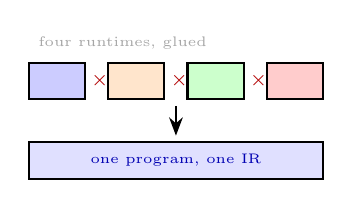
\begin{tikzpicture}[scale=0.84, every node/.style={font=\tiny}, >=Stealth]
				\node[anchor=west, text=gray!70] at (0,2.45) {four runtimes, glued};
				\foreach \x/\c in {0/blue!20, 1.2/orange!20, 2.4/green!20, 3.6/red!20}{
					\draw[thick, fill=\c] (\x,1.6) rectangle (\x+0.85,2.15);
				}
				\foreach \x in {1.075, 2.275, 3.475}{
					\node[text=colWarnLine, font=\scriptsize\bfseries] at (\x,1.875) {$\times$};
				}
				\draw[->, thick] (2.225,1.5) -- (2.225,1.05);
				\draw[thick, fill=colODE] (0,0.4) rectangle (4.45,0.95);
				\node[text=colODELine] at (2.225,0.675) {one program, one IR};
			\end{tikzpicture}
		\end{column}
		\begin{column}{0.32\textwidth}
			\centering
			% 2. The AD tape survives every module boundary
			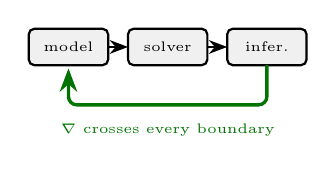
\begin{tikzpicture}[scale=0.84, every node/.style={font=\tiny}, >=Stealth]
				\foreach \x/\l in {0/model, 1.5/solver, 3.0/infer.}{
					\draw[thick, rounded corners=2pt, fill=gray!12]
						(\x,1.6) rectangle (\x+1.2,2.15);
					\node at (\x+0.6,1.875) {\l};
				}
				\draw[->, thick] (1.2,1.875) -- (1.5,1.875);
				\draw[->, thick] (2.7,1.875) -- (3.0,1.875);
				% The backward pass as one unbroken path: out of the inference
				% block, back along the chain, into the model block.
				\draw[->, very thick, green!45!black, rounded corners=3pt]
					(3.6,1.6) -- (3.6,1.0) -- (0.6,1.0) -- (0.6,1.55);
				\node[text=green!45!black] at (2.1,0.62) {$\nabla$ crosses every boundary};
			\end{tikzpicture}
		\end{column}
		\begin{column}{0.32\textwidth}
			\centering
			% 3. One slot, interchangeable modules
			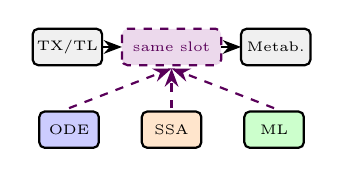
\begin{tikzpicture}[scale=0.84, every node/.style={font=\tiny}, >=Stealth]
				\draw[thick, rounded corners=2pt, fill=gray!12] (0,1.6) rectangle (1.05,2.15);
				\node at (0.525,1.875) {TX/TL};
				\draw[thick, dashed, colPostLine, fill=colPost, rounded corners=2pt]
					(1.35,1.6) rectangle (2.85,2.15);
				\node[text=colPostLine] at (2.1,1.875) {same slot};
				\draw[thick, rounded corners=2pt, fill=gray!12] (3.15,1.6) rectangle (4.2,2.15);
				\node at (3.675,1.875) {Metab.};
				\draw[->, thick] (1.05,1.875) -- (1.35,1.875);
				\draw[->, thick] (2.85,1.875) -- (3.15,1.875);
				\foreach \x/\l/\c in {0.55/ODE/blue!20, 2.1/SSA/orange!20, 3.65/ML/green!20}{
					\draw[thick, rounded corners=2pt, fill=\c]
						(\x-0.45,0.35) rectangle (\x+0.45,0.9);
					\node at (\x,0.625) {\l};
					\draw[->, thick, dashed, colPostLine] (\x,0.95) -- (2.1,1.55);
				}
			\end{tikzpicture}
		\end{column}
	\end{columns}
	\vspace{1mm}
\end{frame}

% ----------------------------------------------------------------
% CUT (Aug 2026): "Which Predictions Can You Trust?" (robust vs fragile
% posterior bands) sat here. It restated motivation rather than advancing the
% argument: slide 3 already pushes a distribution through the forward model, and
% whether that distribution is a prior or a posterior does not change the
% operation being shown. Do not reinstate it in the main line. The content
% survives in build/build_deck.py:slide_trust if it is ever wanted for Q&A.
%
% ALSO CUT (Aug 2026): "One Graph, Two Inference Regimes". Its two dynamics
% sketches were the load-bearing part and now open the test-cell slide below,
% colour-matched to the blocks they imply. Its data-in/blocks/boundary/
% posterior-out flow diagram was dropped: the test-cell schematic next to it
% drew the same partition, so the deck paid twice for one idea.
% ----------------------------------------------------------------



% ================================================================
% SECTION 4: What This Looks Like in Practice
% ================================================================
\section{In Practice}




% ----------------------------------------------------------------
% The landing opens here. The two dynamics sketches came off the retired "One
% Graph, Two Inference Regimes" slide and are deliberately colour-matched to the
% schematic beside them: blue curve -> DifferentiableBlock, orange staircase ->
% SimulationBlock. That mapping was left implicit while the two lived on
% separate slides; here it is the whole point of the layout.
% Rebuilt Aug 2026 around the bursty-regulator cell (BurstyGeneExpression),
% replacing the StochasticGeneExpression harness whose SSA module was the same
% four reactions as the ODE TX/TL block. This one is three distinct subsystems:
% metabolism and enzyme expression are state-coupled both ways (the enzyme gates
% ATP production, mRNA drives the TX/TL sinks), and the regulator is
% parameter-coupled to expression through the shared ribosomes and shared
% degradation machinery. So "cell" is now honest and the retitle is reverted.
%
% Bullets cut Aug 2026 -- the slide is the figure for now. The last one used to
% be a QUESTION, not a goal, and it set up the conditioned-vs-unconditioned
% contrast on the results slide that follows. If the bullets come back, keep
% that pairing; if they stay cut, ask the question out loud instead.
% Layout: schematic LHS (wide column), the two dynamics sketches RHS.
% See docs/superpowers/specs/2026-08-06-minimal-cell-boundary-figure-design.md.
\begin{frame}{A Minimal Cell, in Three Modules}


	\vspace{0.5mm}
	\begin{columns}[T,onlytextwidth]
		\begin{column}{0.60\textwidth}
			\centering
			% No scale= key, and all coordinates in cm: TikZ scales positions but
			% not node minimum widths, so under the old scale=0.50 the two 2.4cm
			% module boxes sat 1.9cm apart and overlapped, crushing the coupling
			% arrow between them. Block labels are named nodes rather than label=
			% options so the outer "test cell" border can fit over them too.
			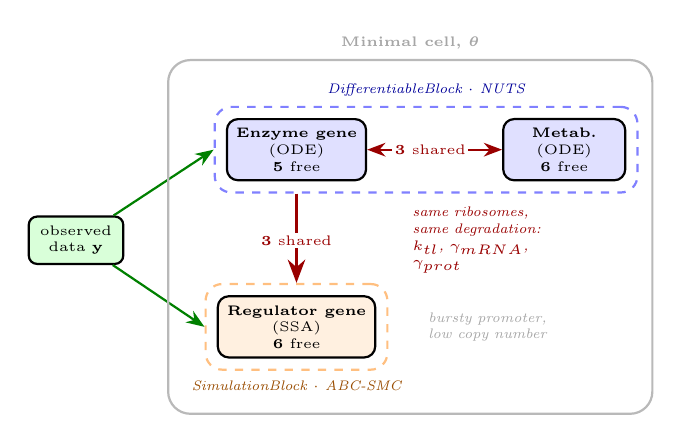
\begin{tikzpicture}[
				mod/.style={draw, thick, rounded corners=4pt, minimum height=0.62cm,
					minimum width=1.55cm, align=center, font=\tiny},
				blk/.style={draw, dashed, thick, rounded corners=6pt, inner sep=4pt},
				>=Stealth
			]
				% Per-box free-parameter counts and per-arrow shared counts, so the
				% "11 unique parameters" arithmetic is checkable on screen:
				% 5 + 6 + 6 = 17, minus 3 shared inside the block, minus 3 across
				% the boundary, = 11. Counts are free parameters as the code counts
				% them (fixed initial conditions excluded, sigma_obs INCLUDED --
				% it is free and it deduplicates between the two ODE modules).
				% Biological rates alone would read 4 / 5 / 6 and 10 unique; if the
				% spoken number is ever changed to 10, change these too.
				%
				% Boxes moved out to +-1.7 from +-1.15: at 1.15 the 1.55cm-wide boxes
				% left a 0.75cm gap, and the "3 shared" label swallowed the arrow
				% whole. 1.7 leaves ~1.8cm, enough for label plus visible shaft.
				%
				% Two-headed arrow because the coupling really is two-way: the
				% enzyme protein gates ATP production (Michaelis-Menten, see
				% LightMetabolism.dynamics) and mRNA drives the TX/TL sinks. That
				% closed loop is what makes these two modules one differentiable
				% block rather than two things solved in sequence.
				\node[mod, fill=blue!12] (txl) at (-1.7,0)
					{\textbf{Enzyme gene}\\(ODE)\\\textbf{5} free};
				\node[mod, fill=blue!12] (met) at (1.7,0)
					{\textbf{Metab.}\\(ODE)\\\textbf{6} free};
				% k_tx, k_tl and sigma_obs are declared by both -- metabolism
				% consumes NTP/AA at the same transcription and translation rates
				% that drive expression. This sharing is INSIDE the block: the joint
				% NUTS fit absorbs it, it never crosses a boundary. Drawn plainly
				% rather than in boundary red for that reason.
				\draw[<->, thick, red!60!black] (txl) -- (met);
				\node[font=\tiny, text=red!60!black, fill=white, inner sep=1pt]
					at (0,0) {\textbf{3} shared};
				\node[blk, blue!50, fit=(txl)(met)] (diffblock) {};
				\node[font=\tiny\itshape, text=blue!60!black, anchor=south]
					(difflab) at (diffblock.north) {DifferentiableBlock $\cdot$ NUTS};

				% A genuinely different subsystem, not the ODE block in another
				% formalism: BurstyGeneExpression carries a two-state promoter
				% (states [promoter, mRNA, protein]; k_on, k_off, k_tx_burst) that
				% has no counterpart upstream. Only k_tl, gamma_mRNA and
				% gamma_protein deduplicate against the enzyme gene -- 3 of 11.
				\node[mod, fill=orange!12] (ssa) at (-1.7,-2.25)
					{\textbf{Regulator gene}\\(SSA)\\\textbf{6} free};
				\node[blk, orange!50, fit=(ssa)] (simblock) {};
				\node[font=\tiny\itshape, text=orange!60!black, anchor=north]
					(simlab) at (simblock.south) {SimulationBlock $\cdot$ ABC-SMC};

				% Sits right of the SSA box, the one empty region inside the cell
				% border at this height: the theta_shared label is at y=-1.15 and
				% simlab is below the block, so nothing competes. Deliberately not in
				% the (cell) fit list -- it already falls inside that border.
				\node[font=\tiny\itshape, text=gray!70, anchor=west, align=left,
					text width=2.0cm] at (-0.15,-2.25)
					{bursty promoter,\\ low copy number};

				% THE boundary. Same count as the intra-block arrow above, but a
				% different kind of sharing: these three are the only route by
				% which anything the differentiable block learns can reach the
				% simulation block. Count verified against the two constructors.
				\draw[->, very thick, red!60!black] (diffblock.south -| ssa) -- (simblock.north);
				\node[font=\tiny, text=red!60!black, fill=white, inner sep=1pt]
					at (-1.7,-1.15) {\textbf{3} shared};
				% Names the physical mechanism rather than the sampler step: the
				% regulator is translated by the same ribosomes and cleared by the
				% same machinery, so these are literally the same three numbers.
				% Explicit breaks: at this width LaTeX hyphenates "ribosomes".
				\node[font=\tiny\itshape, text=red!60!black, anchor=west, align=left,
					text width=2.1cm] at (-0.35,-1.15)
					{same ribosomes,\\ same degradation:\\
					$k_{tl}$, $\gamma_{mRNA}$, $\gamma_{prot}$};

				% y, named where it enters. One arrow into each block because that is
				% what actually happens: both blocks are conditioned on data. A single
				% arrow into the cell would draw the joint conditioning that is still
				% the goal rather than the implementation.
				%
				% x=-4.5, not -3.6: the module boxes are wider than their 1.55cm
				% minimum ("Regulator gene" sets the width), so the fitted cell
				% border reaches further left than the nominal coordinates suggest.
				% At -3.6 the border and both green arrows crossed straight through
				% this node's text. Re-check this clearance if the boxes are ever
				% moved or relabelled -- it is not visible at slide size, only when
				% zoomed.
				\node[draw, thick, rounded corners=3pt, fill=green!15, font=\tiny,
					align=center, minimum width=1.2cm, minimum height=0.5cm]
					(data) at (-4.5,-1.15) {observed\\data $\mathbf{y}$};
				\draw[->, thick, green!50!black] (data) -- (diffblock.west);
				\draw[->, thick, green!50!black] (data) -- (simblock.west);

				% The whole harness, so the three modules read as one system. The
				% data node sits outside it on purpose -- it is not part of the model.
				% Node still named (cell) so the annotation coordinates above and any
				% future .north/.west references keep working; only the caption moved.
				\node[draw, thick, rounded corners=8pt, gray!55, inner sep=5pt,
					fit=(diffblock)(difflab)(simblock)(simlab)] (cell) {};
				\node[font=\tiny\bfseries, text=gray!70, anchor=south]
					at (cell.north) {Minimal cell, $\boldsymbol{\theta}$};
			\end{tikzpicture}
		\end{column}
		\begin{column}{0.38\textwidth}
			\centering
			{\scriptsize\bfseries\color{blue!70!black} Differentiable dynamics}\\[-2pt]
			{\tiny ODE metabolism \& expression, continuous kinetics}\\[1pt]
			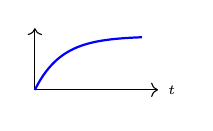
\begin{tikzpicture}[scale=0.34]
				\draw[->] (0,0) -- (4.6,0) node[right, font=\tiny] {$t$};
				\draw[->] (0,0) -- (0,2.3);
				\draw[thick, blue] plot[smooth, domain=0:4] (\x, {2*(1-exp(-\x))});
			\end{tikzpicture}\\[-1pt]
			{\tiny gradients exist $\;\Rightarrow\;$ \textbf{NUTS}}

			\vspace{2.5mm}
			{\scriptsize\bfseries\color{orange!70!black} Stochastic dynamics}\\[-2pt]
			% "Bursty" is now correct: this deck's cell uses BurstyGeneExpression,
			% a telegraph promoter (k_on/k_off gating k_tx_burst) with visible
			% Fano > 1. The staircase below is drawn with bursts for that reason.
			{\tiny Gillespie SSA, bursty promoter, discrete counts}\\[1pt]
			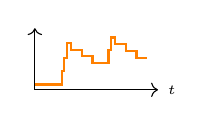
\begin{tikzpicture}[scale=0.34]
				\draw[->] (0,0) -- (4.6,0) node[right, font=\tiny] {$t$};
				\draw[->] (0,0) -- (0,2.3);
				% Bursty, not a random walk: long flat stretches with the promoter
				% off, punctuated by tight runs of up-steps while it is on, then
				% slow decay. That silhouette is the whole reason this module
				% cannot be replaced by its mean-field limit, so it should be
				% legible from the back of the room. Was a generic staircase.
				\draw[thick, orange] (0,0.2) -- (1.0,0.2)
					-- (1.0,0.7) -- (1.1,0.7) -- (1.1,1.2) -- (1.2,1.2)
					-- (1.2,1.75) -- (1.35,1.75)
					-- (1.35,1.5) -- (1.75,1.5) -- (1.75,1.25) -- (2.15,1.25)
					-- (2.15,1.0) -- (2.75,1.0)
					-- (2.75,1.5) -- (2.85,1.5) -- (2.85,1.95) -- (3.0,1.95)
					-- (3.0,1.7) -- (3.4,1.7) -- (3.4,1.45) -- (3.8,1.45)
					-- (3.8,1.2) -- (4.2,1.2);
			\end{tikzpicture}\\[-1pt]
			{\tiny no gradient path $\;\Rightarrow\;$ \textbf{ABC-SMC}}
		\end{column}
	\end{columns}

	% Spends the band the cut bullets left behind, and hands off to the next two
	% slides, which are the two answers. Keep it a question -- the old "Goal: the
	% joint posterior" phrasing promised something the result does not deliver.
	\vfill
	\centering
	{\small \textbf{Goal}: compute $p(\theta | y)$\par}
	\vspace{1mm}
\end{frame}


% ----------------------------------------------------------------
% Results, rebuilt Aug 2026 for the bursty-regulator cell. Supersedes the
% step3 (StochasticGeneExpression) figures, whose simulation module shared ALL
% FOUR of its parameters with the differentiable block because it was the same
% four reactions. That made the old green collapse dramatic but unattributable:
% presented as a boundary result between distinct modules it claimed a transfer
% effect the experiment had not tested, and "how many parameters do the two
% blocks share?" was a one-question refutation. Here it is 3 of 11 and the
% figure shows the transfer stopping at the coupling.
%
% Figure: figures/isab_ssa_posteriors.png, from
%   test/run_talk_bursty_boundary.jl        (compute -> CSV)
%   figures/plot_bursty_boundary.py         (CSV -> figure)
% Parameter ORDER in that figure is load-bearing: the three unshared parameters
% (k_on, k_off, k_tx_burst) come first and the three shared ones (k_tl,
% gamma_mRNA, gamma_protein) last, so the tightening is confined to the
% bottom-right block and the dashed box sits exactly on the coupling. If the
% export order changes, the plot script warns and drops the box rather than
% drawing a wrong one -- check the log before trusting a regenerated figure.
%
% Counts (11 unique, 3 shared) are from the two model constructors:
% BurstyGeneExpression contributes k_on, k_off, k_tx_burst on top of the
% differentiable block's 8; k_tl, gamma_mRNA and gamma_protein deduplicate.
%
% Superseded figures kept in figures/ for Q&A: step3_ssa_posteriors.png (the
% all-four-shared version), step3_corner*.png, step4_corner_talk_shared.png.
%
% MEASURED NUMBERS (job 15152954, 400 particles / 6 populations / 50 replicates
% / 1000 NUTS). Conditioned vs unconditioned, mean +/- sd, sd ratio:
%   k_tl          truth 2.0   4.502+/-3.430 -> 2.074+/-0.086    40x   SHARED
%   gamma_mRNA    truth 0.5   0.437+/-0.403 -> 0.514+/-0.031    13x   SHARED
%   gamma_protein truth 0.1   0.384+/-0.328 -> 0.098+/-0.002   187x   SHARED
%   k_on          truth 0.2   2.106+/-1.979 -> 2.494+/-2.031   0.97x
%   k_off         truth 0.5   0.998+/-1.080 -> 0.893+/-0.883    1.2x
%   k_tx_burst    truth 10.0  5.109+/-4.445 -> 4.259+/-1.447    3.1x
%
% ANTICIPATED QUESTION -- "your promoter rates miss truth, is the SSA inference
% broken?" No, and the answer is worth having ready because it is the
% identifiability claim from slide 8 showing up unprompted. The summary
% statistics are replicate-MEAN trajectories, and a telegraph promoter enters
% the mean only through the effective burst rate
% k_tx_burst * k_on/(k_on + k_off). The individual rates are therefore not
% identifiable from this data at all; the combination is, and it is recovered:
%   truth 2.857   unconditioned 3.307 +/- 2.986   conditioned 2.793 +/- 0.244
% So the boundary sharpens that combination 12x as well. This is why the slide
% says "cannot separate them anyway" rather than claiming they are unconstrained.
% Individual promoter rates would need distributional summaries (Fano factor,
% autocorrelation), not means -- a genuine next step, not a bug.
%
% NOTE: the deck does not state anywhere -- main line or backup -- that the
% computed object is a cut posterior rather than the joint, nor the coverage
% result behind that (the iterative boundary protocol covered truth on 35-70% of
% seeds at a nominal 95%, so single-pass is the default). The setup slide now
% asks a question this result answers honestly, rather than promising the joint
% posterior, so the gap is smaller than it was -- but if the caveat is wanted
% explicitly, an Open Questions slide is where it belongs, phrased as the
% coupling question; step4_calibration_curve.png is still in figures/.
% One figure, not two. The 8-parameter NUTS corner that used to share this slide
% is a methods check, not the argument, and it now lives in backup ("Is the
% Differentiable Half Identifiable?"). A corner plot is square, so on a 16:9
% frame a single one leaves half the width free -- spent here on a plain-language
% read of the figure, which is what a mixed board needs and what a second corner
% was crowding out.
%
% The right column is the spoken argument in three beats: what changed, why
% those three, why not the others. Do not add a fourth.
%
% SPLIT Aug 2026 into two frames -- the setup (each block, its own sampler) and
% the result (the posterior becomes the prior).
%
% The setup slide shows BOTH independent fits side by side, not just the SSA
% one. That is the whole argument made visually: two posteriors, computed by two
% samplers, sitting next to each other with nothing passing between them. The
% ODE corner earns its place because ODE_SUBSET is k_tx plus exactly the three
% SHARED parameters -- so the three tight columns on the left are literally the
% three that are broad inside the box on the right. Point at one, then the
% other; that is the slide.
%
% Consequence: slides 11 and 12 are no longer a pixel-aligned build (the SSA
% corner is smaller on 11 to make room). It is now a zoom-in instead -- same
% figure, larger, with the green added.
%
% To regenerate the figures, from the repo root (the particle CSVs live in
% examples/results, written by job 15152954; that directory is gitignored, so on
% a fresh checkout the run has to be repeated):
%
%   python3 dev/talks/ISAB/figures/plot_bursty_boundary.py --mode ode
%   python3 dev/talks/ISAB/figures/plot_bursty_boundary.py --mode alone
%   python3 dev/talks/ISAB/figures/plot_bursty_boundary.py --mode ssa
%   python3 dev/talks/ISAB/figures/plot_bursty_boundary.py --mode burst
%
% Regenerate ALL FOUR together after any palette change -- burst draws from the
% same constants and backup slide 17 goes stale with the rest.
%
% alone and ssa must come from the SAME particles or slides 11 and 12 disagree.
% ----------------------------------------------------------------
% Beat 1 of 2. The point is NOT "ABC-SMC failed" -- both samplers did exactly
% what they should. The point is that k_tl, gamma_mRNA and gamma_prot get fitted
% twice, by two calculations that never exchange a number, and the second fit is
% far worse than the first. That waste is what the next slide recovers.
%
% Asymmetric columns on purpose: the ODE corner is 4x4 and stays legible small,
% the SSA corner is 6x6 and is the one the next slide zooms into, so it gets the
% extra width.
\begin{frame}{One Way: Each Block, Its Own Sampler}
	\vspace{-2mm}
	% [b], not [c]: the two corners are different heights (4x4 vs 6x6), and
	% centring them puts the two captions at different y, which reads as a
	% misalignment rather than a size difference. Bottom-aligning lines the
	% captions up and lets the corners differ in height, which is the honest
	% cue -- the right-hand posterior is the bigger object.
	\begin{columns}[b,onlytextwidth]
		\begin{column}{0.43\textwidth}
			\centering
			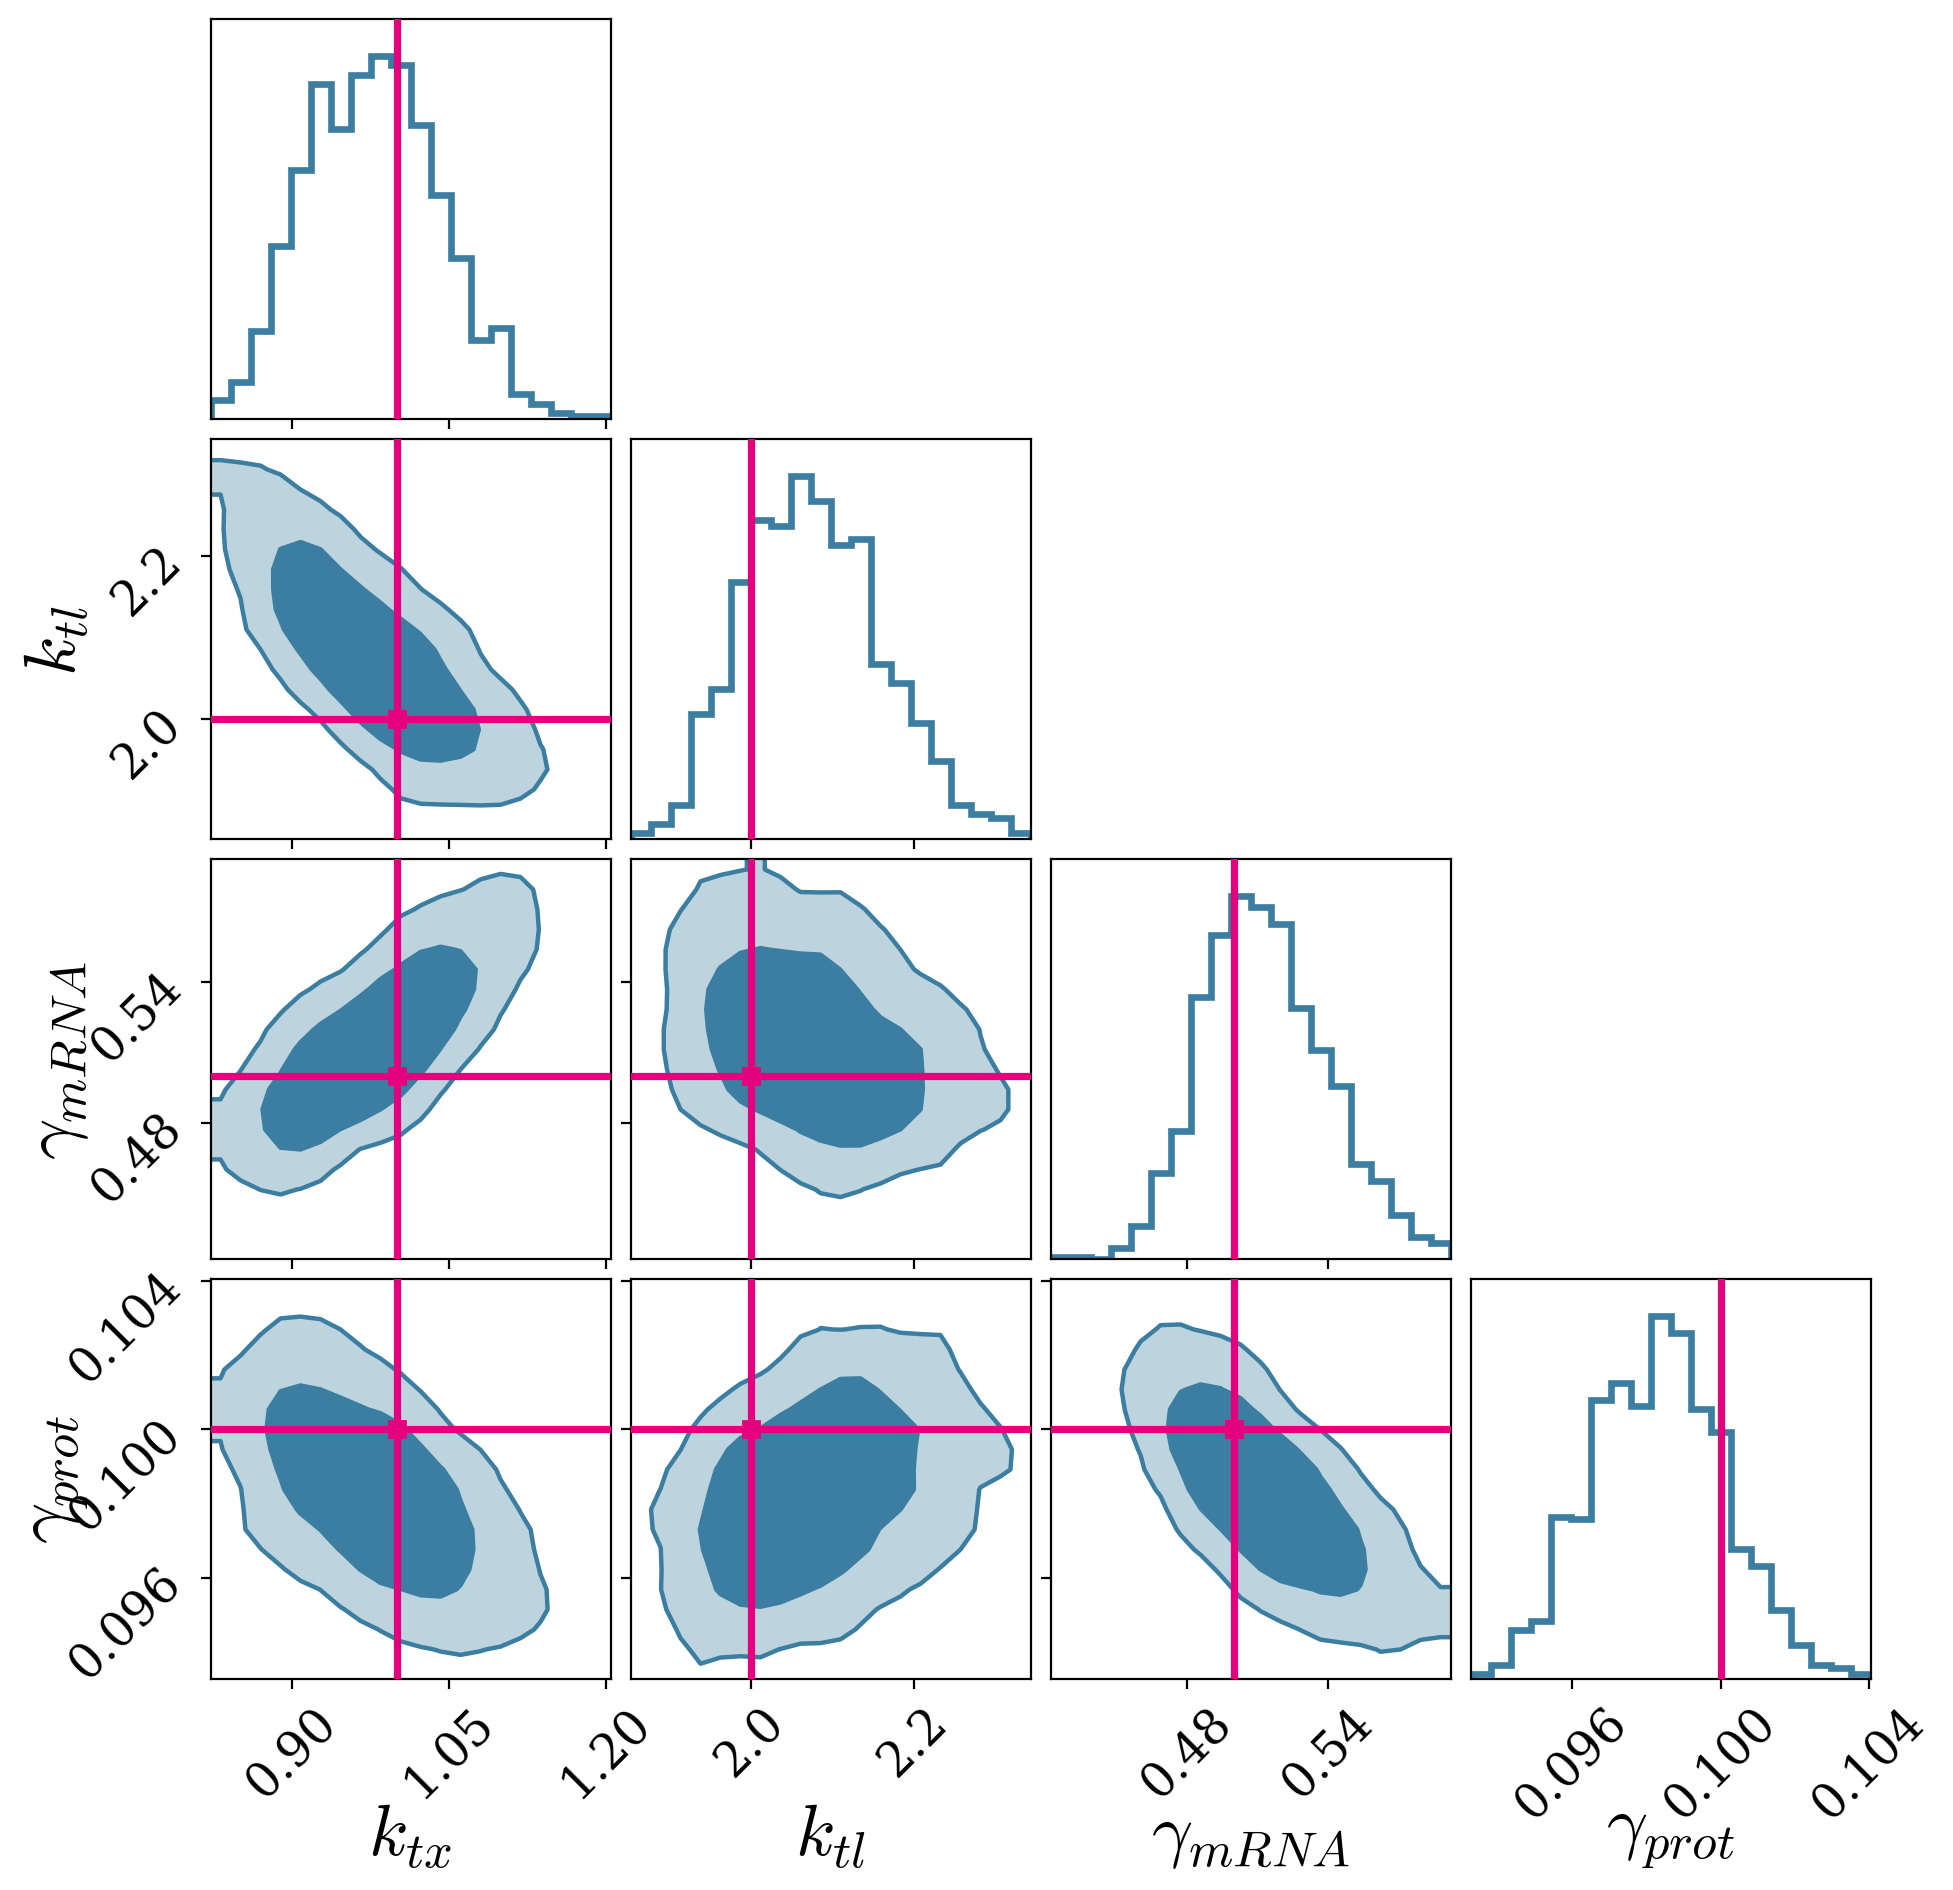
\includegraphics[height=4.7cm]{figures/isab_ode_corner.png}\\[1mm]
			{\scriptsize{\color{figDiff}$\blacksquare$}~\textbf{Differentiable
			block} $\cdot$ NUTS\par}
			{\tiny all 8 parameters jointly, 4 rates shown\par}
		\end{column}
		\begin{column}{0.53\textwidth}
			\centering
			% Falls back rather than failing to build: the particle CSVs live on
			% the cluster (job 15152954) and are not in the repo, so this export
			% cannot be regenerated on a laptop. The placeholder is deliberately
			% loud -- showing the overlay figure here instead would spoil the
			% reveal on the next slide, and quietly.
			\IfFileExists{figures/isab_ssa_alone.png}{%
				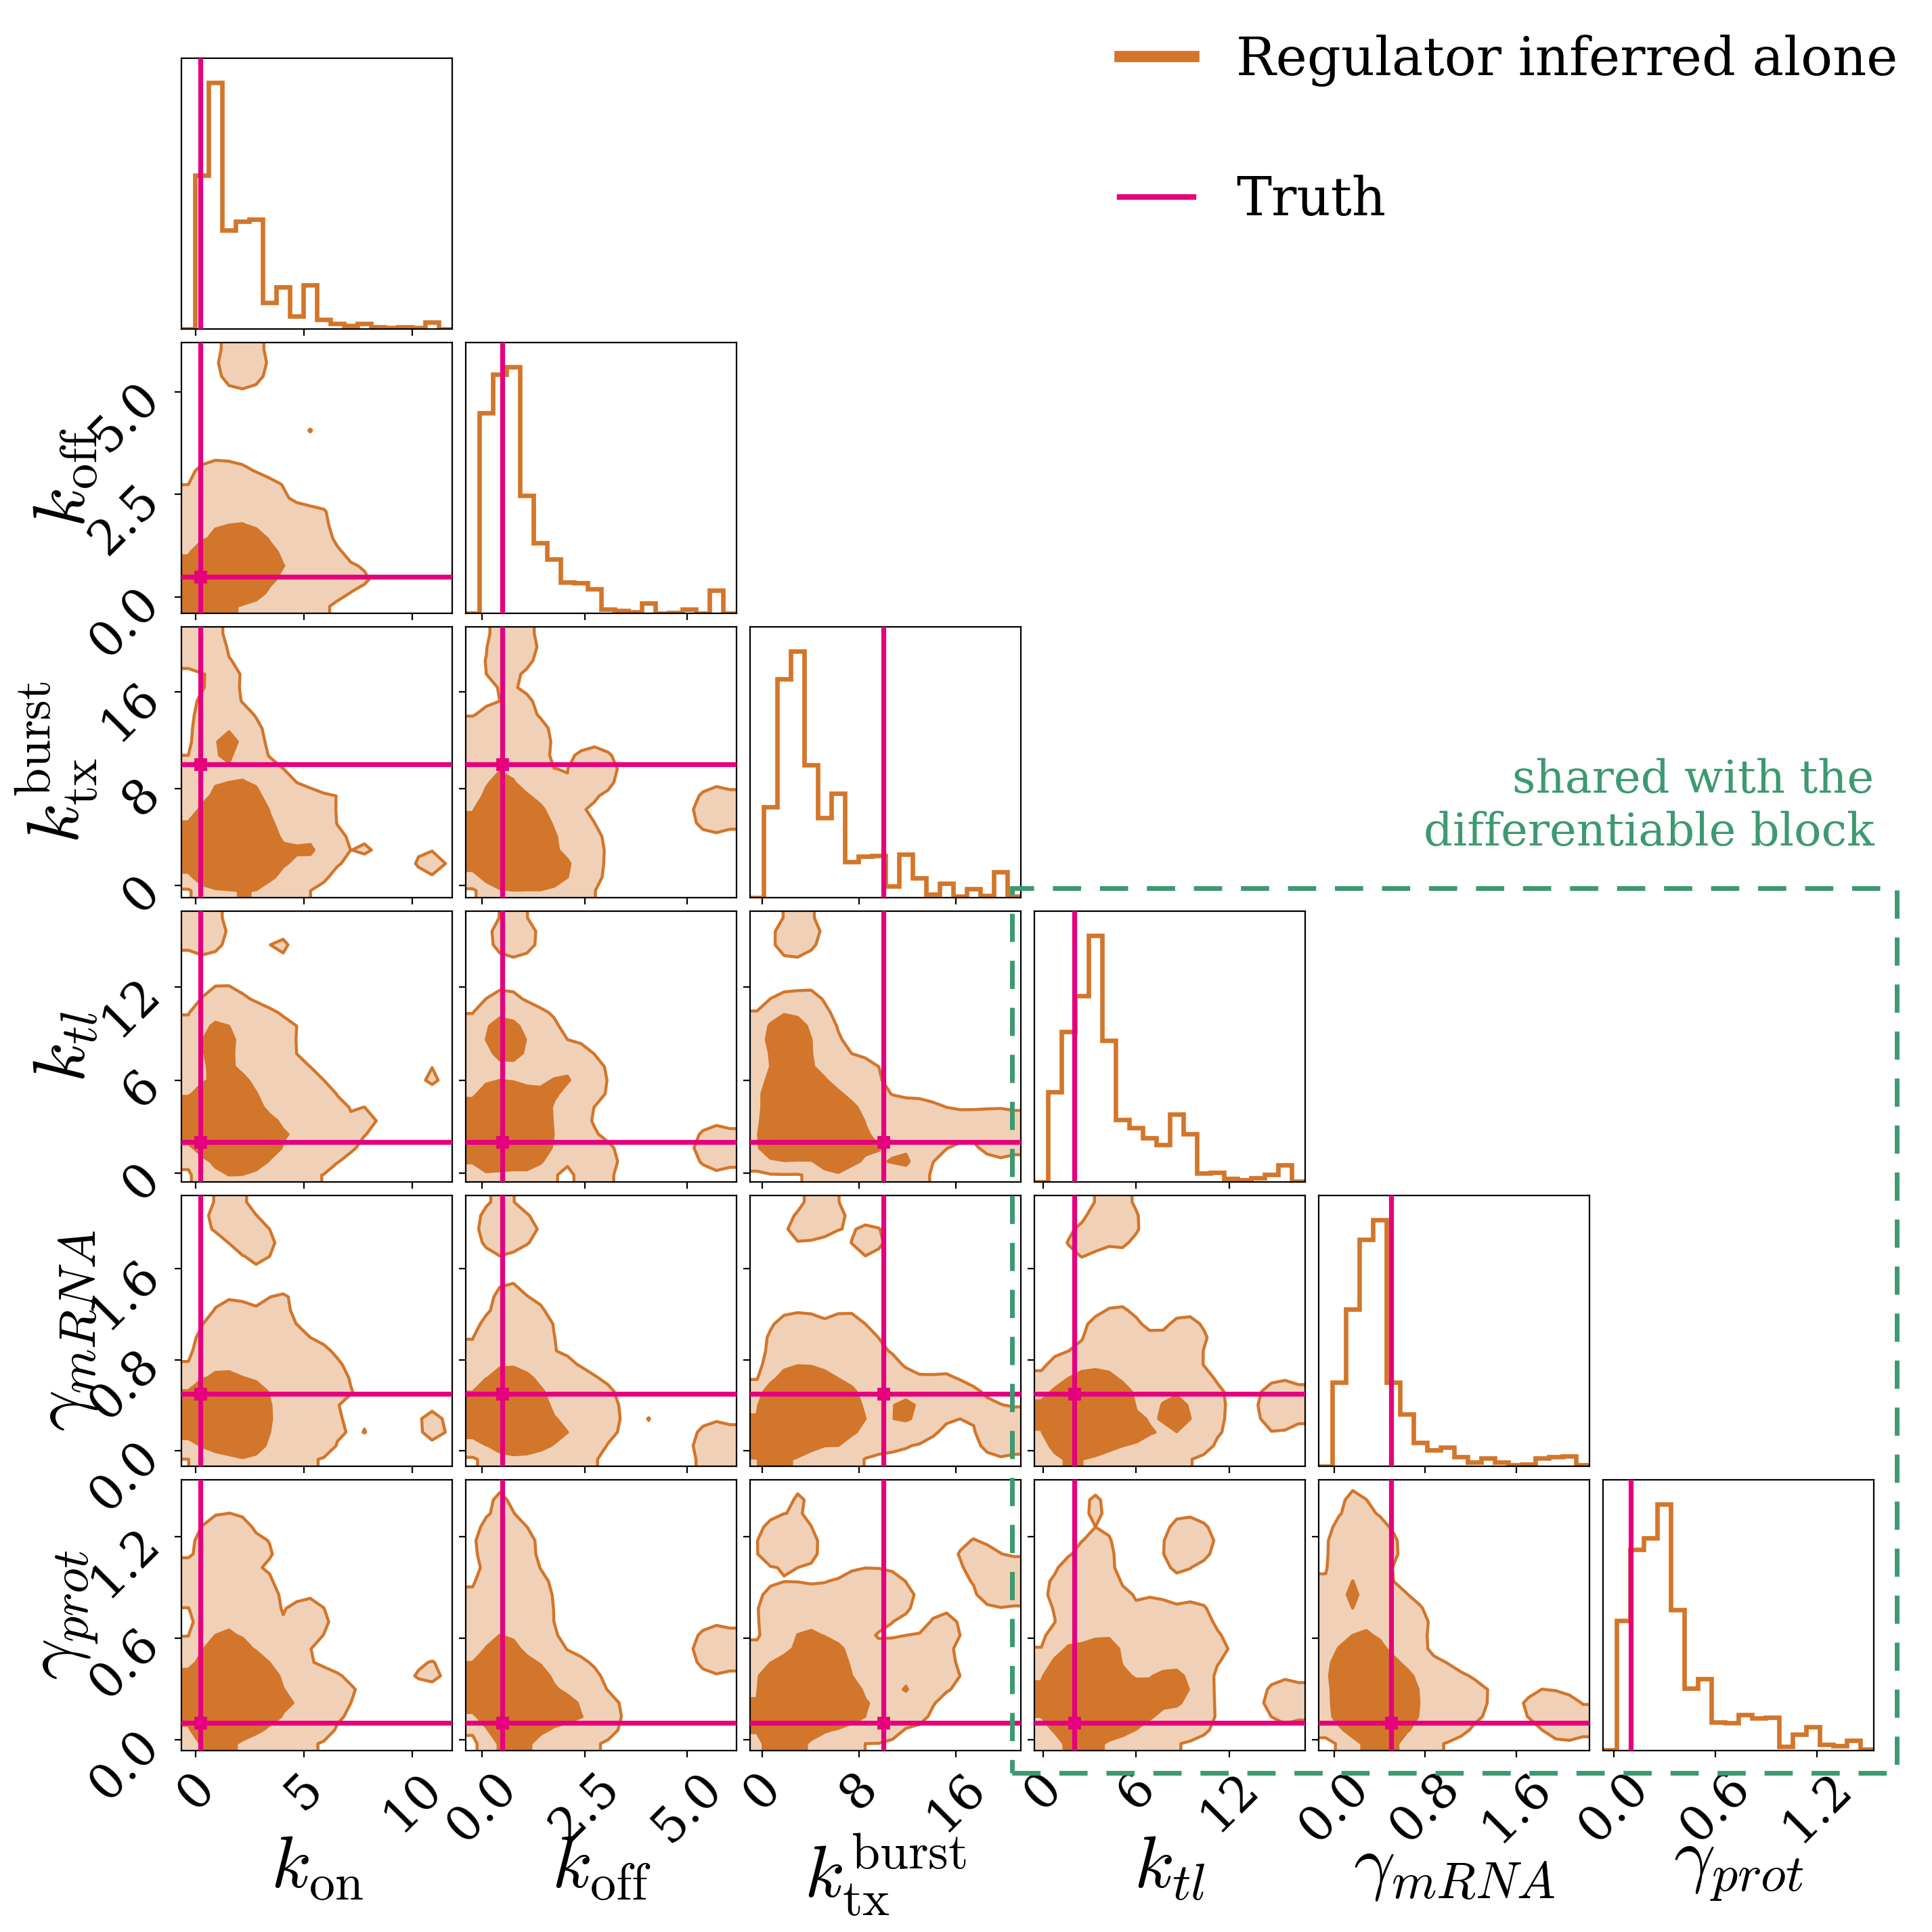
\includegraphics[height=5.5cm]{figures/isab_ssa_alone.png}%
			}{%
				\fbox{\begin{minipage}[c][5.2cm][c]{0.90\linewidth}
					\centering\footnotesize\color{red!70!black}
					\textbf{FIGURE PENDING}\\[2mm]
					{\scriptsize Run \texttt{plot\_bursty\_boundary.py
					-{}-mode alone}\\ against the run's particle CSVs
					(\texttt{examples/results}).\par}
				\end{minipage}}%
			}\\[1mm]
			{\scriptsize{\color{figAlone}$\blacksquare$}~\textbf{Regulator}
			$\cdot$ ABC-SMC\par}
			{\tiny its own data, its own priors\par}
		\end{column}
	\end{columns}

	% The waste, stated as waste. This is the sentence the green answers.
	\vspace{1mm}
	\centering
	{\footnotesize Both calculations are correct --- and
	$k_{tl}$, $\gamma_{mRNA}$, $\gamma_{prot}$ are fitted \textbf{twice},
	by two calculations that never exchange a number.\par}
\end{frame}

% ----------------------------------------------------------------
% Beat 2 of 2. Same figure, green added.
%
% SAY OUT LOUD, do not put on the slide (the board does not need the machinery,
% but the claim should not be overstated either): the flow is ONE-WAY, the
% differentiable block's posterior into the regulator's prior, and nothing the
% regulator's data knows travels back. This is a cut posterior, a principled
% approximation to the joint rather than the joint itself. If asked whether it
% is exact: no, and the framework makes the gap measurable -- the iterative
% protocol covered truth on 35-70% of seeds at a nominal 95%, which is why
% single-pass is the default here. step4_calibration_curve.png is in figures/.
\begin{frame}{Another Way: let information flow between modules}
	\vspace{-1mm}
	\begin{columns}[c,onlytextwidth]
		\begin{column}{0.60\textwidth}
			\centering
			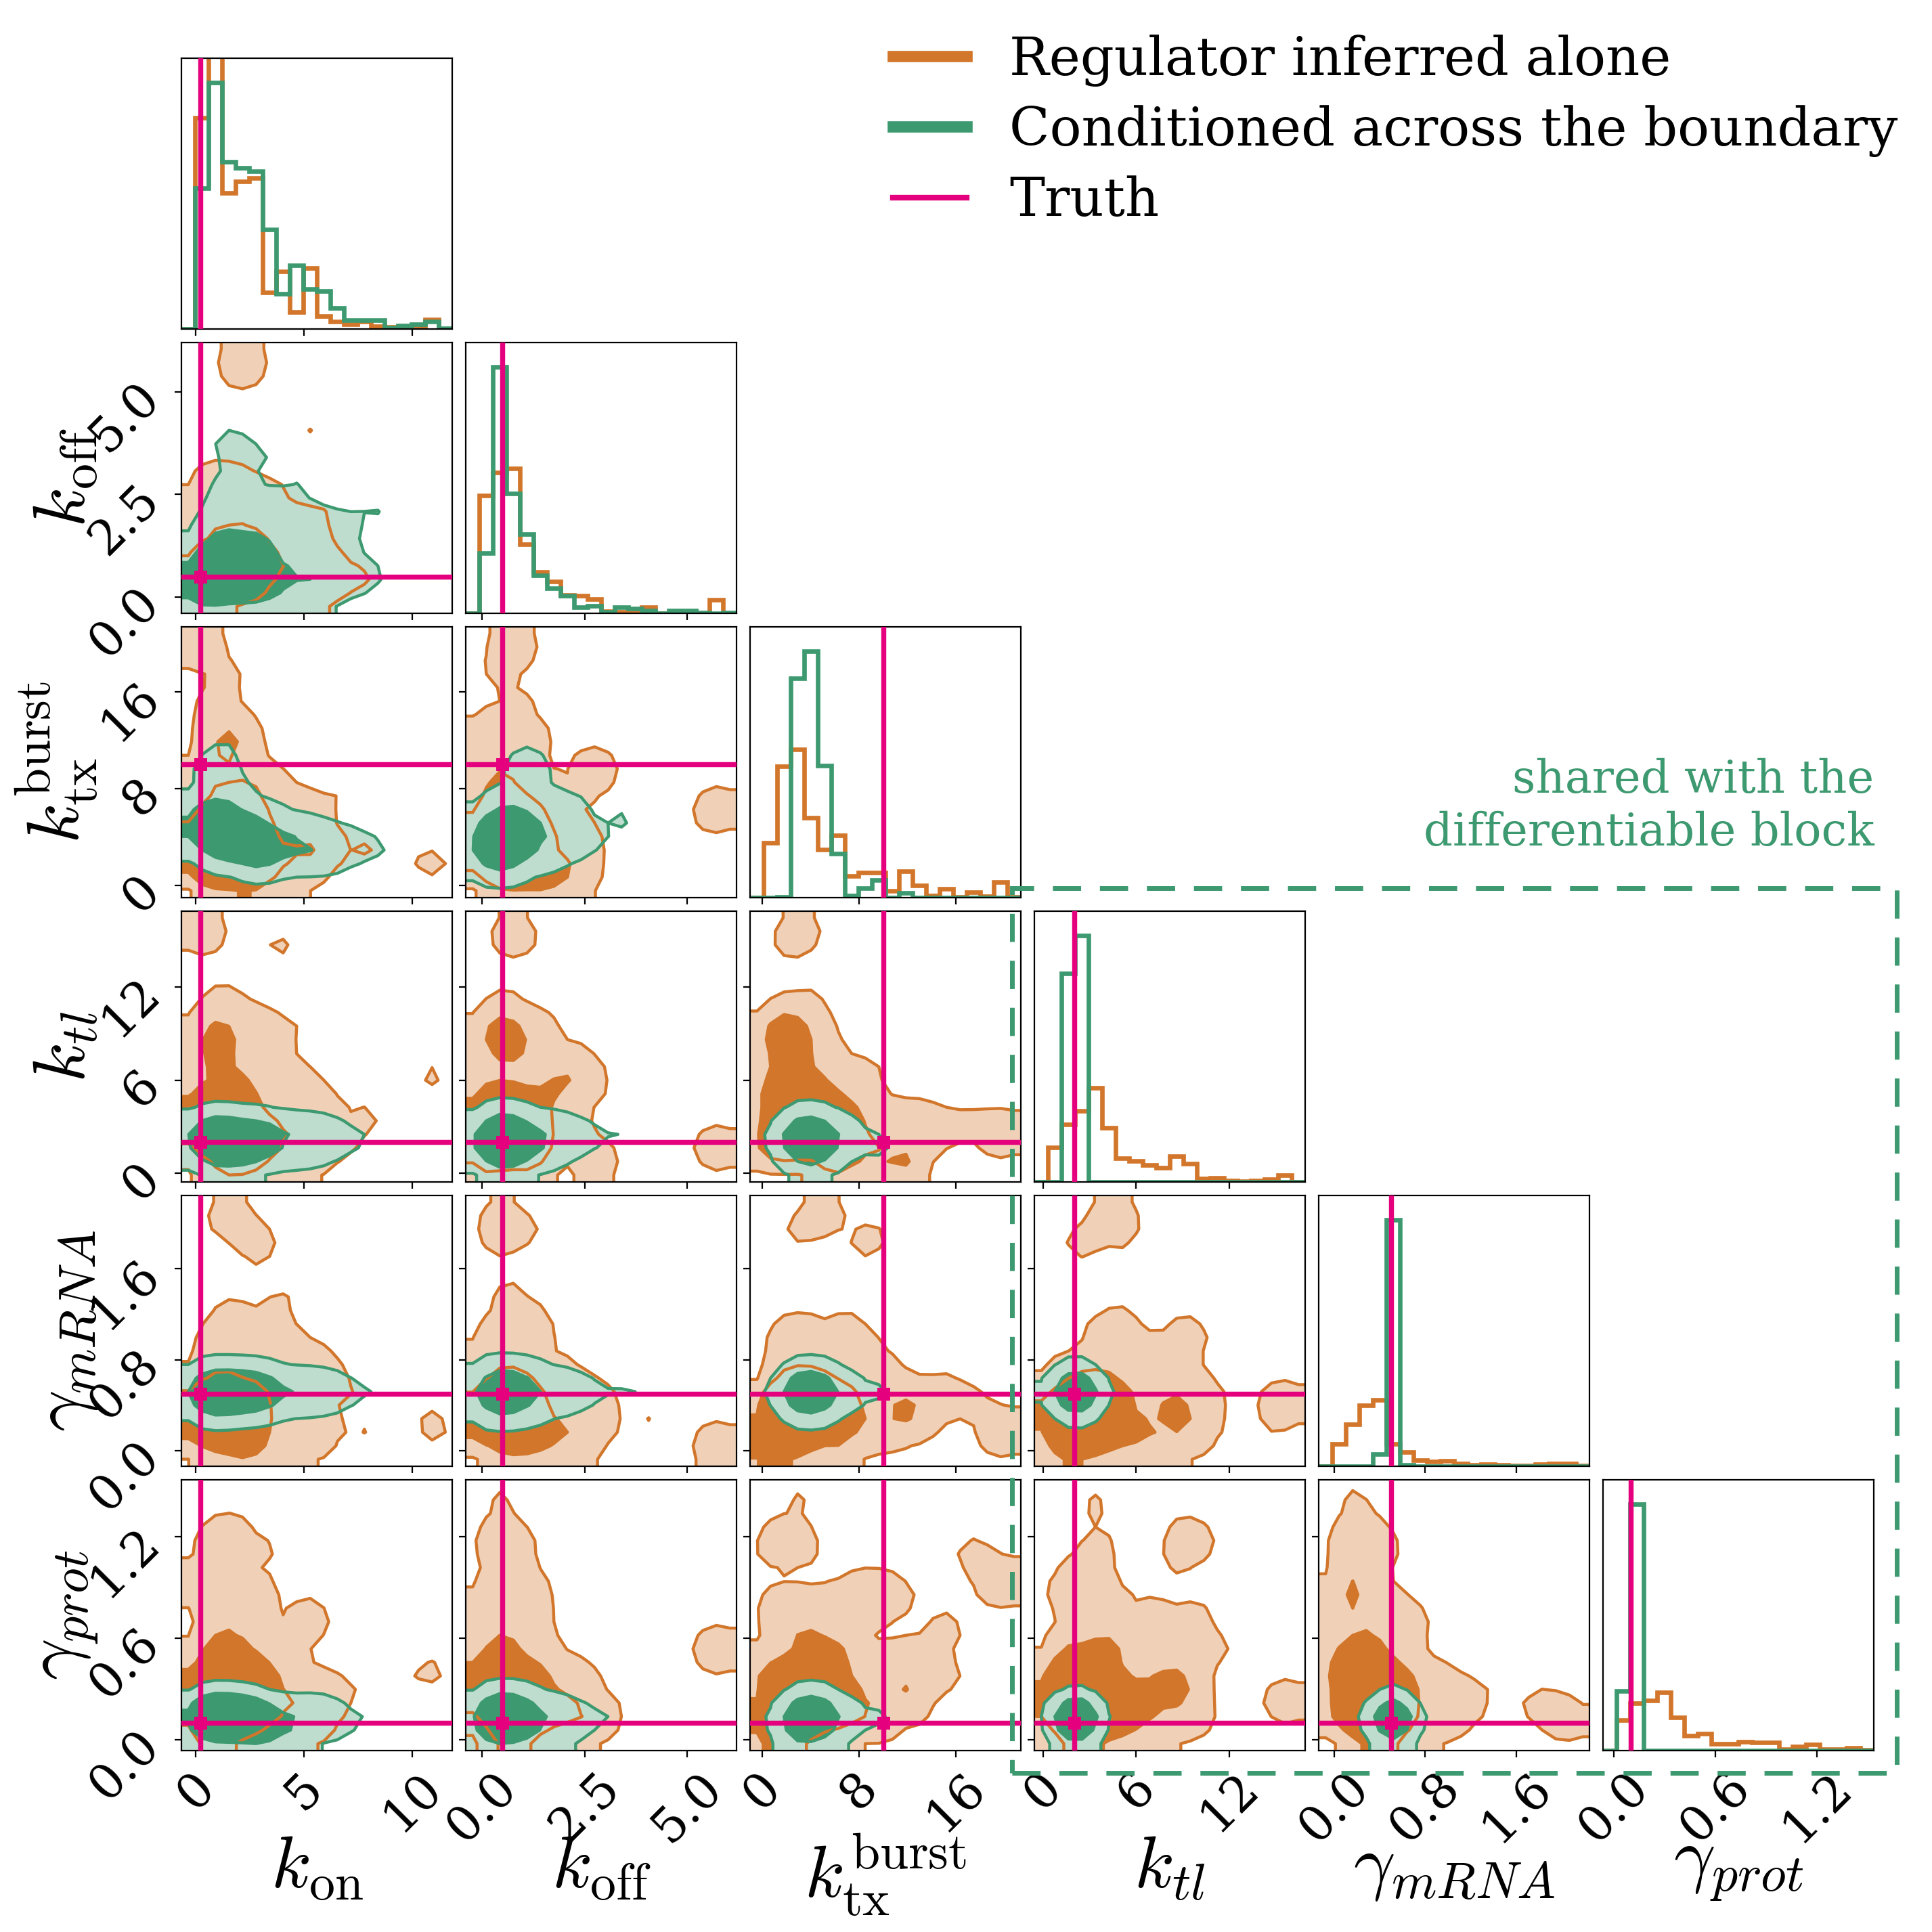
\includegraphics[height=6.4cm]{figures/isab_ssa_posteriors.png}
		\end{column}
		% \footnotesize and bare paragraphs rather than \small and an itemize: at
		% 0.38\textwidth the fuller version overran the frame top and bottom.
		% Keep it to these four beats if it is edited again.
		\begin{column}{0.38\textwidth}
			\footnotesize
			{\color{figCond}$\blacksquare$}~\textbf{Conditioned} --- the
			shared parameters now carry the differentiable block's posterior
			across the boundary as their prior.

			\smallskip
			{\color{figAlone}$\blacksquare$}~\textbf{Alone}, from the previous
			slide, for comparison.

			\medskip
			$\rightarrow$~The \textbf{3 boxed} parameters sharpen onto truth:
			exactly the 3 the expression modules share.

			% NOT "barely move": k_tx_burst tightens 3.1x despite never being
			% conditioned, because the six are fitted jointly and it is correlated
			% with the pinned parameters (corr +0.36 with gamma_prot, -0.24 with
			% k_tl). k_on and k_off are near-uncorrelated and genuinely do not
			% move. "Indirectly" covers both honestly.
			\smallskip
			$\rightarrow$~The other 3 govern \textbf{promoter switching}. They keep
			their own priors and move only \textbf{indirectly}, through the
			likelihood --- and mean trajectories cannot separate them anyway.

			\medskip
			% "Reached as far as the coupling carried it", not "stopped where the
			% coupling stopped": the bullet above now says the unshared parameters
			% move indirectly, so a hard stop would contradict it one line later.
			{\scriptsize\itshape Information crossed the boundary --- and reached
			as far as the coupling carried it.\par}
		\end{column}
	\end{columns}
\end{frame}

% ----------------------------------------------------------------
% Redrawn Aug 2026 as a funnel, replacing three equal prose columns plus a
% sandbox band. The shape is the argument: phases 1-2 are a single narrow track
% (one organism, machinery under test), and everything downstream of a validated
% framework fans out at once. Three same-width columns drew phase 3 as merely
% the third of three, which understated it -- what actually happens after
% validation is a branching, not a next step.
%
% The fan carries the rest of slide 8 (model selection, experimental design)
% alongside the two things the board is best placed to react to: other
% organisms, and MACSYS's own experimental data. The sandbox is one branch here
% rather than a band beneath everything: as a band it read as a co-equal north
% star and cost six lines of prose; as a branch it is what it is -- one of the
% options validation buys.
%
% Text is deliberately at chip length. Everything that was prose here is now
% spoken: the syn3A ~1000 literature parameters, "expect tens constrained not
% thousands", and the closing experimentalist loop.
%
% Phase 2 does not name a data source, deliberately: the Open Questions slide
% asks the board which real datasets to condition on, so asserting one here
% would answer our own question.
%
% Geometry: all coordinates in cm with no scale= key -- TikZ scales positions
% but not node minimum widths, so mixing the two pulls the fan apart. Total
% picture width is ~13.7cm against a 14.0cm textwidth; widening the chips past
% 6.4cm overflows the margin.
\begin{frame}{Where This is Going}

	\vspace{1mm}
	\centering
	\begin{tikzpicture}[
		ph/.style={draw, thick, rounded corners=4pt, minimum width=2.6cm,
			minimum height=1.3cm, align=center, font=\tiny, fill=blue!8},
		chip/.style={draw, thick, rounded corners=3pt, minimum width=6.2cm,
			minimum height=0.62cm, align=left, text width=5.85cm, font=\tiny},
		>=Stealth
	]
		% ===== The narrow track =====
		% \\ must not appear inside a braced group in a node with align=: it breaks
		% TikZ's alignment machinery (undefined \tikz@finish@orig at \end{frame}).
		% Hence \textit per line rather than one {\itshape ...} spanning both.
		\node[ph] (p1) at (0,0)
			{{\bfseries\color{oxfordblue}PHASE 1}\\[2pt]
			 \textbf{Recover a known}\\\textbf{injection}\\[2pt]
			 \textit{syn3A: simulate,}\\\textit{infer back, check}};
		\node[ph] (p2) at (2.95,0)
			{{\bfseries\color{oxfordblue}PHASE 2}\\[2pt]
			 \textbf{Condition on}\\\textbf{real data}\\[2pt]
			 \textit{posteriors as output;}\\\textit{identifiability}};
		\draw[->, very thick, oxfordblue] (p1) -- (p2);

		\node[draw, dashed, gray!55, rounded corners=6pt, inner sep=4pt,
			fit=(p1)(p2)] (track) {};
		\node[font=\tiny\itshape, text=gray!70, anchor=north]
			at (track.south) {narrow on purpose: one organism, machinery under test};

		% ===== The gate: what validation buys =====
		% rotate=90 rather than \rotatebox: graphicx's rotation inside a TikZ node
		% breaks pgf's scope bookkeeping (undefined \tikz@finish@orig). The node's
		% own anchors rotate with it, so the fan arrows leave from an explicit
		% coordinate instead of gate.east.
		\node[draw, thick, rounded corners=3pt, fill=oxfordblue, rotate=90,
			minimum width=2.2cm, minimum height=0.55cm, inner sep=2pt,
			font=\tiny\bfseries, text=white] (gate) at (5.05,0)
			{validated framework};
		\coordinate (gateL) at (4.75,0);
		\coordinate (gateR) at (5.35,0);
		\draw[->, very thick, oxfordblue] (track.east) -- (gateL);

		% ===== The fan =====
		\node[chip, fill=orange!14] (c1) at (9.05,2.16)
			{\textbf{Other organisms} --- not just a minimal cell};
		\node[chip, fill=green!16]  (c2) at (9.05,1.08)
			{\textbf{MACSYS data} --- metabolomics, genomics, constructs};
		\node[chip, fill=blue!12]   (c3) at (9.05,0)
			{\textbf{Model selection} --- which mechanism does the data prefer?};
		\node[chip, fill=colPost]   (c4) at (9.05,-1.08)
			{\textbf{Experimental design} --- what to measure next};
		\node[chip, fill=gray!18]   (c5) at (9.05,-2.16)
			{\textbf{Sandbox} --- surrogates, reduced models, cheap solves};

		\foreach \c in {c1,c2,c3,c4,c5}{
			\draw[->, thick, gray!60] (gateR) to[out=0, in=180] (\c.west);
		}

		\node[font=\tiny\bfseries, text=oxfordblue, anchor=south]
			at ([yshift=2pt]c1.north) {PHASE 3 ONWARDS};
	\end{tikzpicture}
\end{frame}






% ================================================================
% SECTION 5: Summary & Outlook
% ================================================================
\section{Summary \& Outlook}

% ----------------------------------------------------------------
% The closing slide, and currently the deck's only one in this section: the Open
% Questions frame below is commented out, so this carries the ask as well as the
% recap. Four items in the order the talk made them --- problem, pivot, evidence,
% ask.
%
% Adapted from the Brisbane deck's Summary (2026-05-brisbane-macsys/talk.tex).
% Two changes from that version. Item 3 is new: Brisbane had no result to report,
% whereas this deck spends two slides on the test cell and the boundary result,
% and a summary that skips its own evidence reads as a proposal rather than a
% progress report. Item 4 replaces "Interested? Get involved!" --- a board's
% currency is advice, data and introductions, and the two asks named are the two
% that slide 12's fan already set up, so they land as a continuation.
%
% Columns 0.64/0.34 with [c]: the pipeline sits on the optical centre of the list
% rather than riding item 1. The diagram is the inference half of slide 5 with
% identical geometry (coordinates in cm, no scale= key --- see there for why); one
% picture the whole talk turns on, so it costs nothing to draw twice.
\begin{frame}{Summary}
	\begin{columns}[c,onlytextwidth]
		\begin{column}{0.68\textwidth}
			\small
			\begin{enumerate}\itemsep3pt
				\item \textbf{The problem.} Whole-cell models take
				${\sim}$1000 parameters from literature and simulate forward. No
				uncertainty quantification, no way to learn from data, no way to
				know which predictions to trust.

				\item \textbf{InferCell inverts the question.} Given
				observations, infer parameters and their uncertainties --- the
				model becomes something you condition on data, not just run
				forward.

				% Names the three modules: by this point the board has seen them
				% once, and the recap is where a general audience fixes what the
				% "cell" actually was. "Where the two share machinery" is the
				% qualifier that keeps this honest -- the boundary sharpened 3 of
				% 11 parameters, not all of them.
				\item \textbf{Toy pilot works.} A three-module minimal cell ---
				metabolism, gene expression, a bursty regulator --- with ODE and
				SSA in one graph. Information crosses the module boundary and
				sharpens the posterior onto truth, where the modules share
				machinery. On synthetic data, so far.

				\item \textbf{What would help most.} Real datasets to condition
				on; a route into organisms beyond a minimal cell.\\[2pt]
				% One line, and short enough to stay one line: the full
				% repo-plus-issues-plus-come-talk-to-me version wrapped and left
				% "issue" orphaned. A board talks to you rather than filing
				% issues, so the issues link is the one to drop.
				{\scriptsize\href{https://github.com/MACSYS-CoE/InferCell}{github.com/MACSYS-CoE/InferCell}}
			\end{enumerate}
		\end{column}
		\begin{column}{0.30\textwidth}
			\centering
			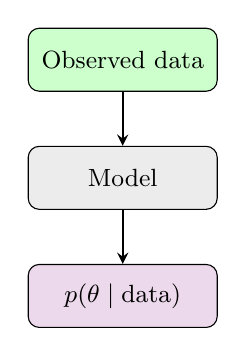
\begin{tikzpicture}
				\node[pipelinebox=green!20, minimum width=2.4cm] (d) at (0,0) {Observed data};
				\node[pipelinebox=gray!15, minimum width=2.4cm] (m) at (0,-1.5) {Model};
				\node[pipelinebox=colPost, minimum width=2.4cm] (p) at (0,-3.0) {$p(\theta \mid \text{data})$};
				\draw[pipelinearr] (d) -- (m);
				\draw[pipelinearr] (m) -- (p);
			\end{tikzpicture}\\[6pt]
			% Explicit break at the comma: at this column width the caption wraps
			% anyway, and left to itself it breaks after "are".
			{\scriptsize\itshape ``Given data,\\ what $\theta$ are consistent?''}
		\end{column}
	\end{columns}
\end{frame}

% ----------------------------------------------------------------
% ----------------------------------------------------------------
% Only genuinely open things belong here, and each is aimed at a seat in the
% room. Board: Possingham (chair, mathematical ecology / decision science),
% Andrews (yeast functional genomics), Lecuit (physics of living systems),
% Silver (synthetic biology), Troyanskaya (ML/genomics), Wishart (metabolomics).
%
% Rewritten Aug 2026. Two questions were retargeted and one replaced:
%
% - Q1 (data) is unchanged in substance: the strongest ask, because Wishart,
%   Andrews and Silver know the syn3A landscape and we do not. Now says
%   explicitly that AVAILABILITY is the part we cannot compute -- asking the
%   board what is worth measuring would undercut the BOED claim on slide 12.
%
% - Q2 replaces "is syn3A the right validation vehicle?", which invited the
%   board to relitigate a decision already justified by tractability (only
%   minimal cell with a published forward simulator and a known injection).
%   Asked forwards instead, it is genuinely open and attaches to the "other
%   organisms" branch of slide 12's fan. The Luthey-Schulten collaboration route
%   is promoted onto the slide: a route in is exactly what a board can supply.
%
% - Q3 is new, replacing "who should we design for?". That one depended mostly
%   on our own capacity, so we were better placed to answer it than the board,
%   and its trilemma was artificial (at v0.1 the users are modellers and methods
%   people regardless). The scope question is instead the objection most likely
%   to arrive from Lecuit unbidden, so it is better invited deliberately.
%
% - Q4 keeps the coupling problem but drops the sampler framing. Nobody here
%   picks between cut, Gibbs and PMCMC (that ladder is a backup slide). Posed as
%   accuracy-for-which-claim it lands on Possingham, whose field is exactly how
%   approximate a model can be and still support a decision. The 35-70% coverage
%   number stays: it is the one measured fact on the slide, and it is what makes
%   this a real question rather than a hedge.
%
% Note the two jobs this slide does. Q1 and Q2 are asks -- we want a dataset, a
% name, a route in, and should push for answers. Q4 is partly a disclosure: its
% value is showing we found the weak point in our own method first. Pace the
% discussion accordingly; do not fish for a fix to Q4.
%
% Headers are kept under ~33 characters so each sets on one line at this column
% width. A wrapped question reads as prose and loses the punch of four clean
% asks.










% ----------------------------------------------------------------
%\begin{frame}{Open Questions}
%	\begin{itemize}\itemsep6pt
%		\item \textbf{Does it scale?}
%		{\small v1 has ${\sim}$9 parameters across 3 modules. Whole-cell models have ${\sim}$2000.}\\
%		{\small\color{gray} Modular design means each inference block stays small. Adjoint sensitivity methods and amortized SBI are the path to scaling parameter count within blocks; the graph structure itself scales by adding modules, not by growing a single sampler.}
%
%		\item \textbf{Why Julia?}
%		{\small The SBI and ML ecosystems live in Python/JAX.}\\
%		{\small\color{gray} Julia's multiple dispatch and AD composability make the modular interface natural. Catalyst.jl provides a CRN DSL with no JAX equivalent. For v1, the contribution is the architecture, not the scale --- Julia lets us express the ideas most directly. If neural SBI becomes critical, a Python bridge is feasible.}
%
%		\item \textbf{What does the hybrid sampler target?}
%		{\small Gluing NUTS and SBI across module boundaries --- is the result the true joint posterior?}\\
%		{\small\color{gray} In general, no --- the cut posterior is an approximation. But the framework provides a spectrum: from fully cut (fast, approximate) through Gibbs to PMCMC (exact, expensive). Diagnosing the gap between levels is a built-in validation step, not an afterthought.}
%
%		\item \textbf{What if the model is wrong?}
%		{\small All models are wrong. Do you get confident-but-wrong posteriors?}\\
%		{\small\color{gray} Posterior predictive checks flag when the model cannot reproduce the data. Comparing posteriors across formalisms (ODE vs SSA) detects structural misspecification. The framework doesn't solve model misspecification, but it makes it visible.}
%	\end{itemize}
%\end{frame}

% ----------------------------------------------------------------






% ================================================================
% BACKUP SLIDES
% ================================================================
\makeatletter
\pdfstringdefDisableCommands{\let\translate\@firstofone}
\makeatother
\appendix
\backupbegin
% ----------------------------------------------------------------
\begin{frame}[noframenumbering]{Backup}
\end{frame}

% ----------------------------------------------------------------
% Moved off the main results slide (Aug 2026). It is a methods check, not the
% boundary argument, and sharing the results slide with the boundary figure made
% that slide answer two questions at once -- the specific thing that made the
% setup-to-results transition read badly. It still pays off the identifiability
% bullet on "What Becomes Possible (Science)", so it is the first backup after
% the divider: reach for it if anyone asks whether the differentiable half
% actually worked.
%
% Same NUTS chain as the main result -- sequential_infer runs the ODE block
% first and unconditioned, so this is that stage, not a separate fit. 4 of the
% 8 parameters shown (see ODE_SUBSET in plot_bursty_boundary.py); the rates
% carry the claim and the 8x8 grid is illegible at slide height.
% Deliberately repeats the main line's left-hand corner rather than replacing
% it. On slide 11 the figure is small and its job is comparative -- tight next
% to broad. Here it is full size and the job is the tilted ellipses, which are
% invisible at slide-11 scale. Same figure, different claim; if this is ever
% cut, move the ellipse point into the main line rather than losing it.
\begin{frame}[noframenumbering]{Is the Differentiable Half Identifiable?}
	\begin{columns}[c,onlytextwidth]
		\begin{column}{0.58\textwidth}
			\centering
			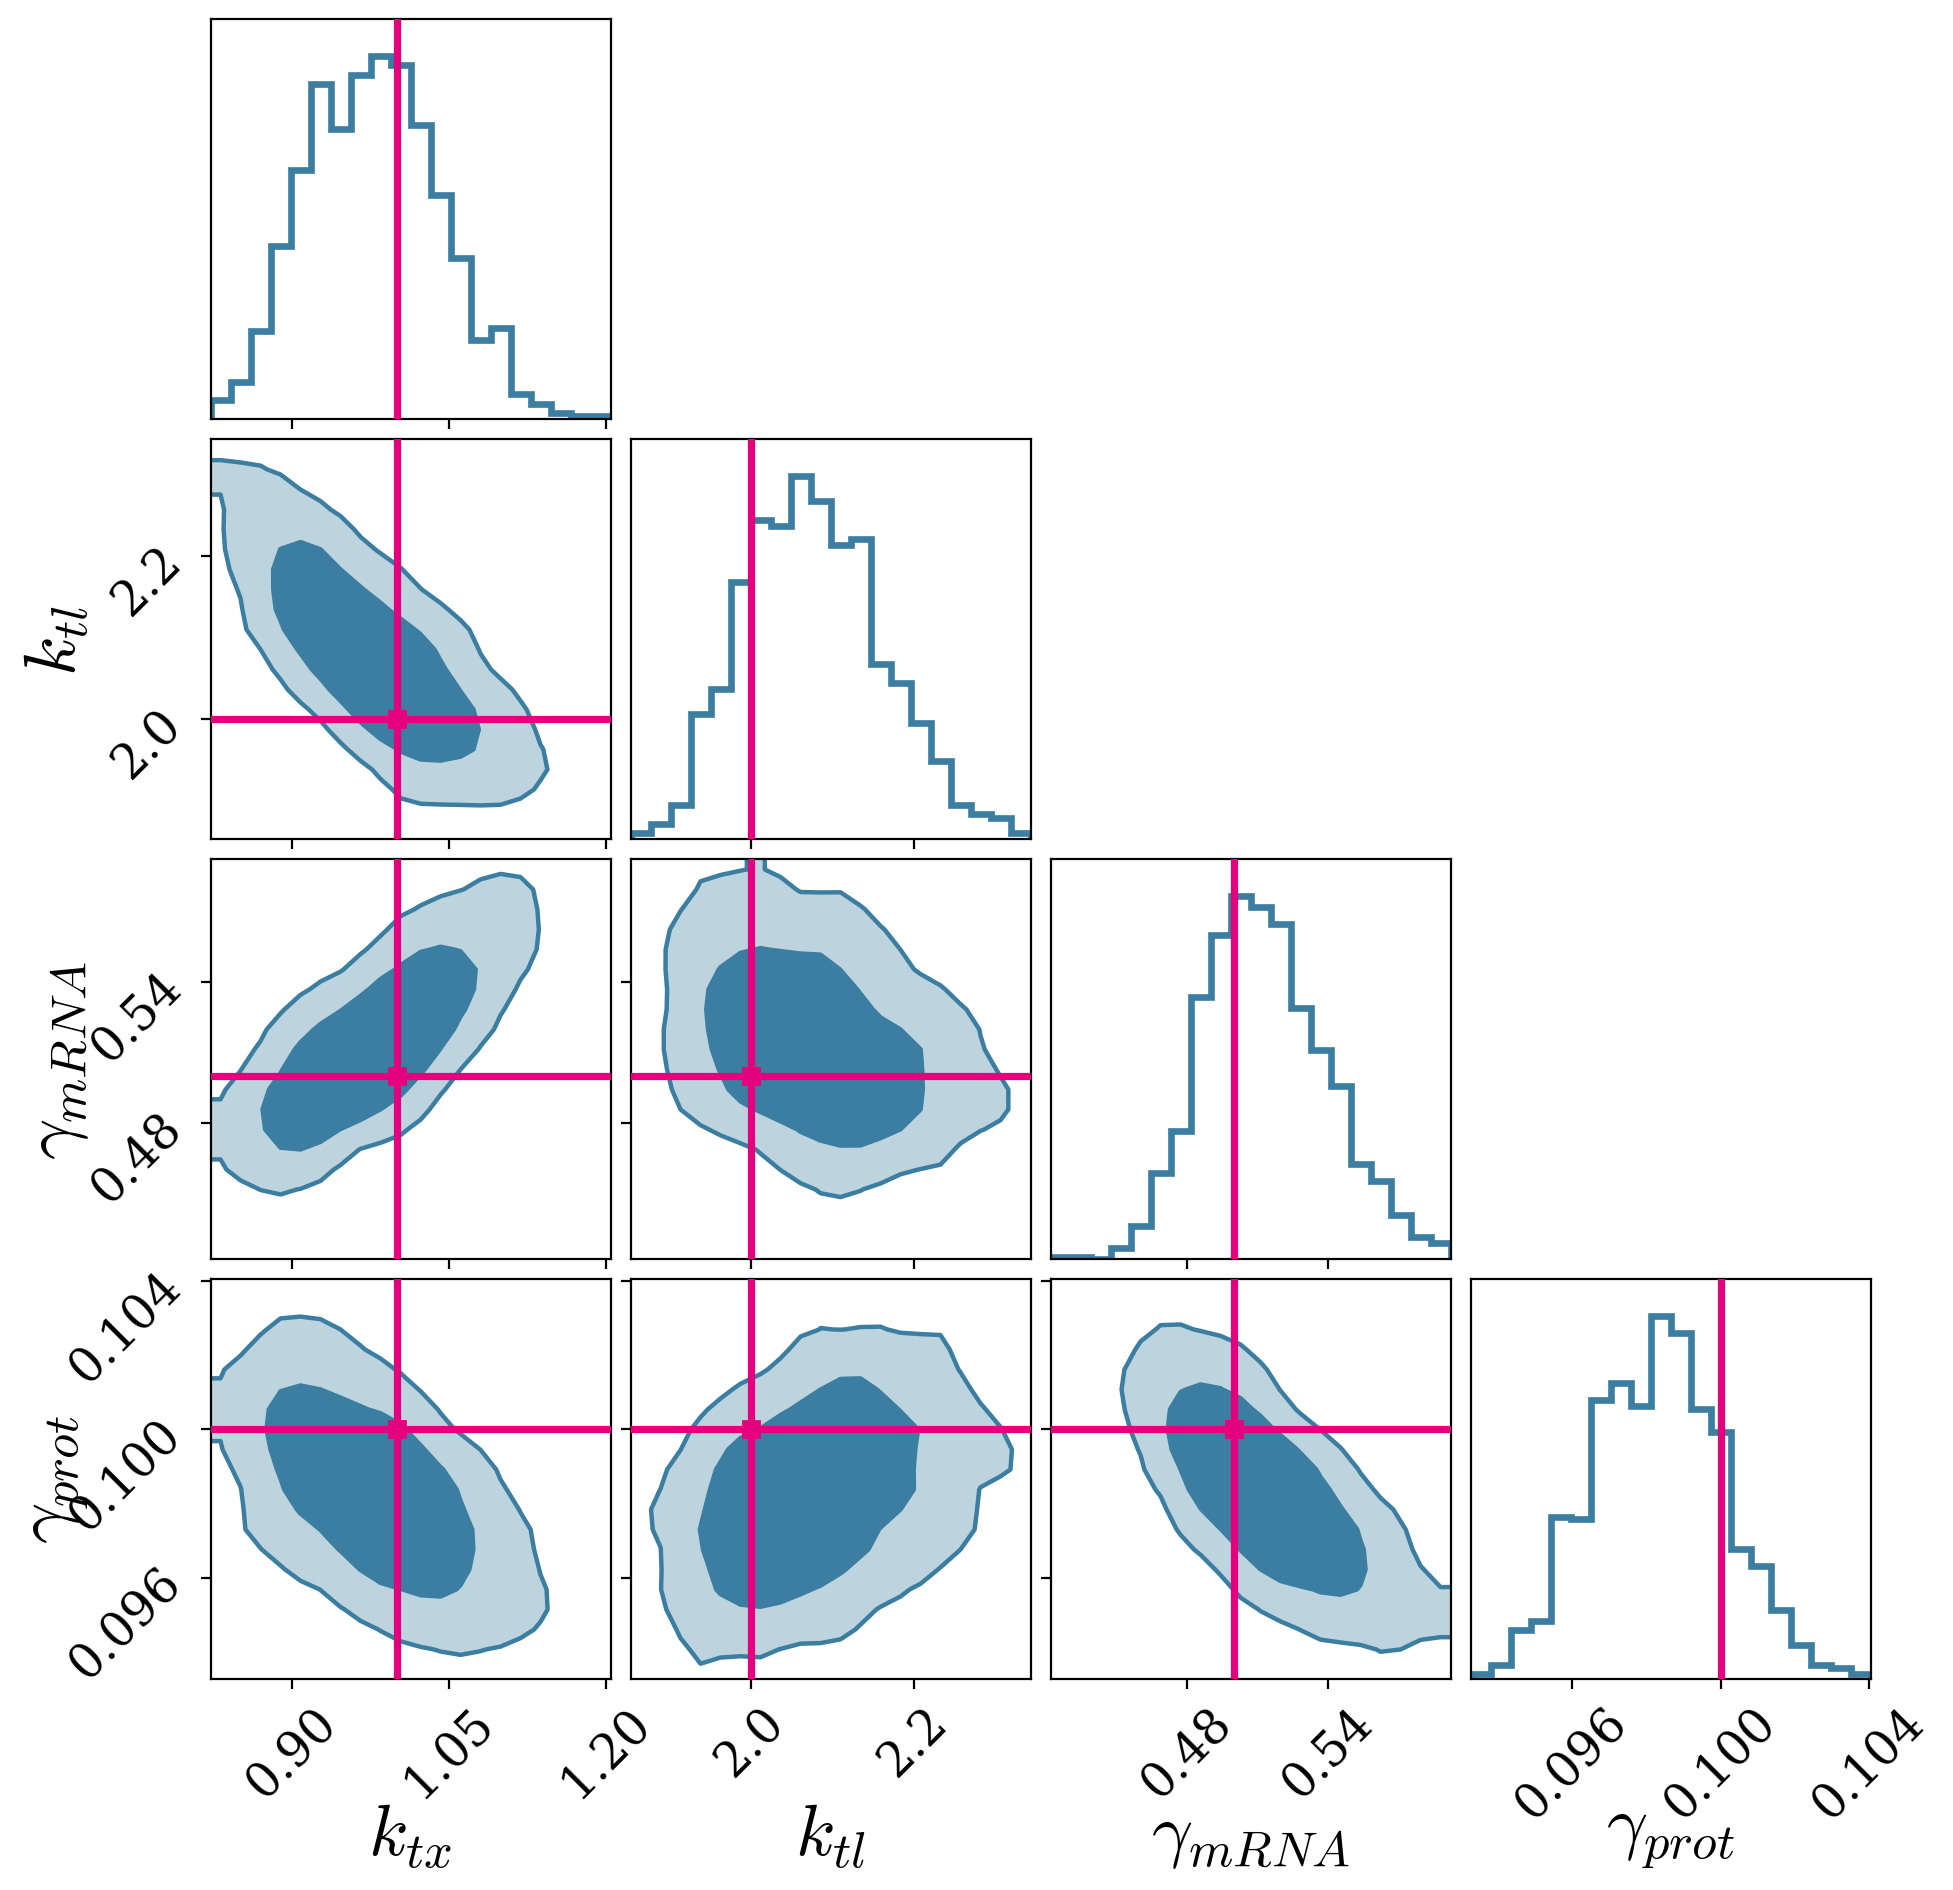
\includegraphics[height=6.2cm]{figures/isab_ode_corner.png}
		\end{column}
		\begin{column}{0.40\textwidth}
			\small
			The left-hand posterior from ``One Way'', full size: joint NUTS over
			the differentiable block, all \textbf{8} parameters at once. 4 rates
			shown.

			\medskip
			\begin{itemize}\itemsep3pt
				\item {\color{figTruth}$\blacksquare$}~Magenta lines mark truth.
				\item \textbf{Tilted ellipses} are the point: the data
				constrains \emph{combinations} of rates, not every rate on its
				own.
			\end{itemize}

			\medskip
			{\scriptsize\itshape Identifiability measured, rather than assumed ---
			one of the questions forward simulation cannot pose.\par}
		\end{column}
	\end{columns}
\end{frame}

% ----------------------------------------------------------------
% The answer to the question the results slide invites. Someone will notice
% that k_on and k_tx_burst sit nowhere near their orange lines and ask whether
% the SSA inference is broken. It is not, and the reason is the identifiability
% claim from "What Becomes Possible (Science)" turning up unprompted -- which is
% a better thing to be asked about than most. Have this slide ready.
%
% Numbers from job 15152954. Figure from
% plot_bursty_boundary.py --mode burst.
\begin{frame}[noframenumbering]{Why Do Three Parameters Miss Truth?}
	\begin{columns}[c,onlytextwidth]
		\begin{column}{0.52\textwidth}
			\centering
			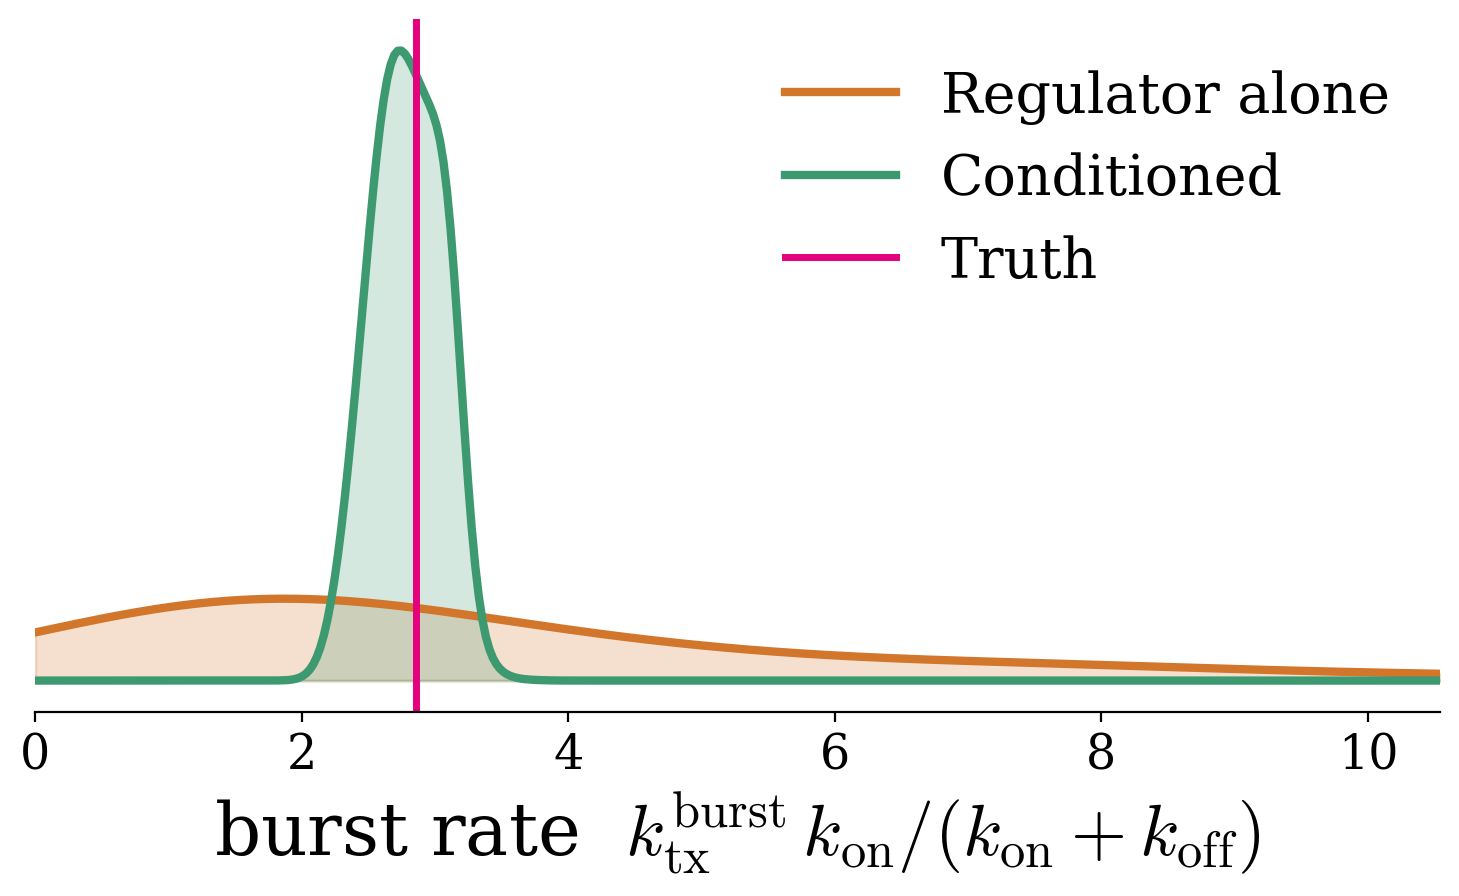
\includegraphics[width=\linewidth]{figures/isab_burst_rate.png}
		\end{column}
		\begin{column}{0.46\textwidth}
			\footnotesize
			The data are replicate-\textbf{mean} trajectories. A telegraph
			promoter enters the mean \emph{only} through the burst rate
			$k_{\mathrm{tx}}^{\mathrm{burst}}k_{\mathrm{on}}/
			(k_{\mathrm{on}}{+}k_{\mathrm{off}})$.

			\smallskip
			So the three rates are \textbf{not individually identifiable} from
			this data --- by either block. Their combination is:

			\smallskip
			\begin{tabular}{@{}ll@{}}
				truth & 2.86\\
				alone & $3.31 \pm 2.99$\\
				conditioned & $\mathbf{2.79 \pm 0.24}$\\
			\end{tabular}

			\smallskip
			The boundary sharpens \emph{that} $12\times$ too --- and it is why
			$k_{\mathrm{tx}}^{\mathrm{burst}}$'s own marginal tightened
			$3\times$ without ever being conditioned.

			\smallskip
			{\scriptsize\itshape Not a broken sampler. An identifiability result
			the framework surfaced on its own.\par}
		\end{column}
	\end{columns}
\end{frame}

% ----------------------------------------------------------------
% Follow-on from the slide above: what we would change to fix it. Worth having
% because it converts the weakness into a concrete next step, and because the
% closing argument here -- if means sufficed, the mean-field ODE would do, so
% the SSA module only earns its place once the summaries see beyond the mean --
% is the sharpest available answer to "why carry a stochastic module at all?".
% That question is likelier from this board than the identifiability one.
\begin{frame}[noframenumbering]{What Would Constrain the Promoter Rates?}
	\small
	Nothing about the model or the sampler --- the \textbf{summary statistics}.

	\medskip
	\begin{columns}[T,onlytextwidth]
		\begin{column}{0.48\textwidth}
			\textbf{What we use now}
			\begin{itemize}\itemsep2pt
				\item Replicate-mean trajectories
				\item Sees the burst rate only
				\item Identical information content to the mean-field ODE
			\end{itemize}
		\end{column}
		\begin{column}{0.48\textwidth}
			\textbf{What would separate the rates}
			\begin{itemize}\itemsep2pt
				\item \textbf{Fano factor} --- bursting pushes it above 1
				\item \textbf{Autocorrelation time} --- sets
				$k_{\mathrm{on}}{+}k_{\mathrm{off}}$
				\item \textbf{Full count distribution} --- higher moments split
				the burst size from its frequency
			\end{itemize}
		\end{column}
	\end{columns}

	\vfill
	\centering
	\alert{\small If the mean were enough, the mean-field ODE would do. The
	stochastic module only earns its place once the summaries look past the
	mean.}
	\vspace{2mm}
\end{frame}

% ----------------------------------------------------------------
\begin{frame}[noframenumbering]{Conditioning the Whole Model}
	\centering
	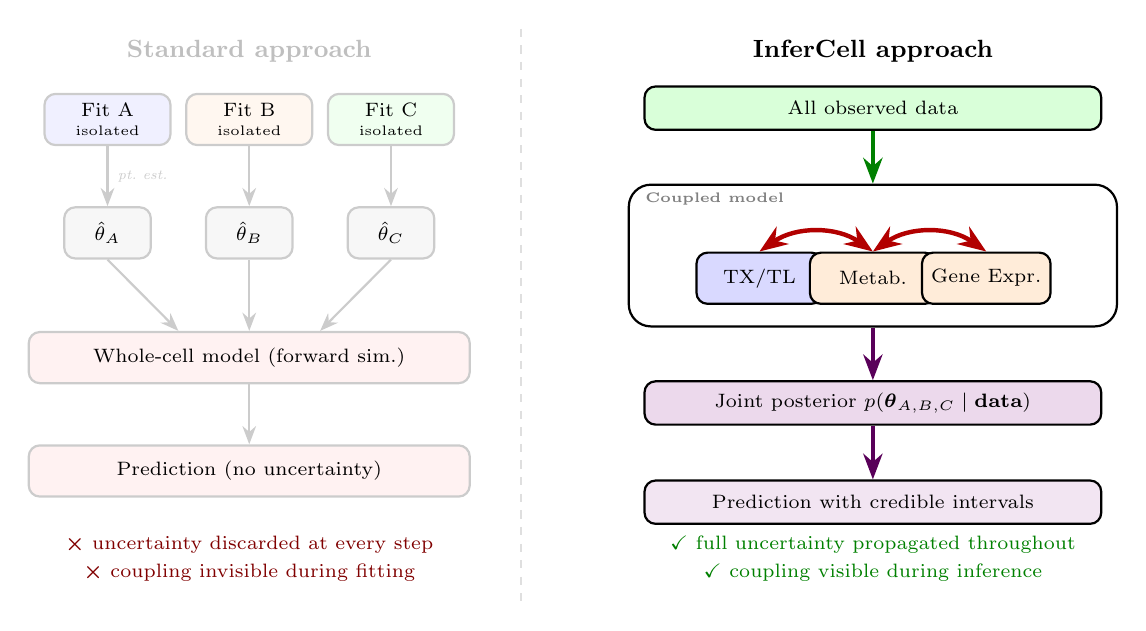
\begin{tikzpicture}[
		scale=0.72,
		mod/.style={draw, thick, rounded corners=4pt, minimum height=0.65cm, align=center, font=\scriptsize},
		>=Stealth
	]
		% ===== LEFT: Standard approach (dimmed) =====
		\node[font=\small\bfseries, text=gray!50] at (-5.5, 5.2) {Standard approach};

		% Isolated fits
		\node[mod, fill=blue!6, draw=gray!40, minimum width=1.6cm] (fA) at (-8, 4.0) {Fit A\\[-1pt]{\tiny isolated}};
		\node[mod, fill=orange!6, draw=gray!40, minimum width=1.6cm] (fB) at (-5.5, 4.0) {Fit B\\[-1pt]{\tiny isolated}};
		\node[mod, fill=green!6, draw=gray!40, minimum width=1.6cm] (fC) at (-3, 4.0) {Fit C\\[-1pt]{\tiny isolated}};

		% Point estimates
		\node[mod, fill=gray!6, draw=gray!40, minimum width=1.1cm] (pA) at (-8, 2.0) {$\hat{\theta}_A$};
		\node[mod, fill=gray!6, draw=gray!40, minimum width=1.1cm] (pB) at (-5.5, 2.0) {$\hat{\theta}_B$};
		\node[mod, fill=gray!6, draw=gray!40, minimum width=1.1cm] (pC) at (-3, 2.0) {$\hat{\theta}_C$};

		\draw[->, thick, gray!40] (fA) -- (pA) node[midway, right, font=\tiny\itshape, text=gray!40] {pt.\ est.};
		\draw[->, thick, gray!40] (fB) -- (pB);
		\draw[->, thick, gray!40] (fC) -- (pC);

		% Assembly
		\node[mod, fill=red!5, draw=gray!40, minimum width=5.6cm] (wcm) at (-5.5, -0.2) {Whole-cell model (forward sim.)};
		\draw[->, thick, gray!40] (pA.south) -- ([xshift=-1.25cm]wcm.north);
		\draw[->, thick, gray!40] (pB) -- (wcm);
		\draw[->, thick, gray!40] (pC.south) -- ([xshift=1.25cm]wcm.north);

		% Output
		\node[mod, fill=red!5, draw=gray!40, minimum width=5.6cm] (out) at (-5.5, -2.2) {Prediction (no uncertainty)};
		\draw[->, thick, gray!40] (wcm) -- (out);

		% Problems
		\node[font=\scriptsize, text=red!50!black] at (-5.5, -3.5) {$\boldsymbol{\times}$ uncertainty discarded at every step};
		\node[font=\scriptsize, text=red!50!black] at (-5.5, -4.0) {$\boldsymbol{\times}$ coupling invisible during fitting};

		% ===== DIVIDER =====
		\draw[thick, gray!25, dashed] (-0.7, 5.6) -- (-0.7, -4.5);

		% ===== RIGHT: InferCell (vivid) =====
		% Layout: equal gaps (~0.97 TikZ units) between all four block edges.
		% Box 1.8cm tall; three small boxes 0.55cm tall; scale=0.72.
		\node[font=\small\bfseries] at (5.5, 5.2) {InferCell approach};

		% Data at top
		\node[draw, thick, rounded corners=4pt, fill=green!15,
			  font=\scriptsize, minimum width=5.8cm, minimum height=0.55cm]
			  (data) at (5.5, 4.2) {All observed data};

		% Coupled model box
		\node[draw, thick, rounded corners=8pt,
			  minimum height=1.8cm, minimum width=6.2cm,
			  fill=white] (cbox) at (5.5, 1.6) {};
		\node[font=\tiny\bfseries, text=gray, anchor=north west]
			  at ([xshift=4pt]cbox.north west) {Coupled model};

		% Modules inside the box
		\node[mod, fill=blue!15, minimum width=1.6cm] (mA) at (3.5, 1.2) {TX/TL};
		\node[mod, fill=orange!15, minimum width=1.6cm] (mB) at (5.5, 1.2) {Metab.};
		\node[mod, fill=orange!15, minimum width=1.6cm] (mC) at (7.5, 1.2) {Gene Expr.};

		% Coupling arrows --- arched above the modules
		\draw[<->, line width=1.6pt, red!70!black] (mA.north) to[bend left=35] (mB.north);
		\draw[<->, line width=1.6pt, red!70!black] (mB.north) to[bend left=35] (mC.north);

		% Data -> coupled model
		\draw[->, line width=1.4pt, green!50!black] (data) -- (cbox);

		% Joint posterior
		\node[draw, thick, rounded corners=4pt, fill=colPost,
			  font=\scriptsize, minimum width=5.8cm, minimum height=0.55cm]
			  (post) at (5.5, -1.0) {Joint posterior $p(\boldsymbol{\theta}_{A,B,C} \mid \textbf{data})$};
		\draw[->, line width=1.4pt, colPostLine] (cbox) -- (post);

		% Prediction with UQ
		\node[draw, thick, rounded corners=4pt, fill=violet!10,
			  font=\scriptsize, minimum width=5.8cm, minimum height=0.55cm]
			  (predR) at (5.5, -2.75) {Prediction with credible intervals};
		\draw[->, line width=1.4pt, colPostLine] (post) -- (predR);

		% Benefits
		\node[font=\scriptsize, text=green!50!black] at (5.5, -3.5) {$\checkmark$ full uncertainty propagated throughout};
		\node[font=\scriptsize, text=green!50!black] at (5.5, -4.0) {$\checkmark$ coupling visible during inference};
	\end{tikzpicture}

\end{frame}

% ----------------------------------------------------------------
\begin{frame}[noframenumbering]{How Much Coupling Do You Need?}
Joint inference over all parameters is intractable. \newline  Isolated submodel fits discard all coupling. 

	\bigskip
	\centering
	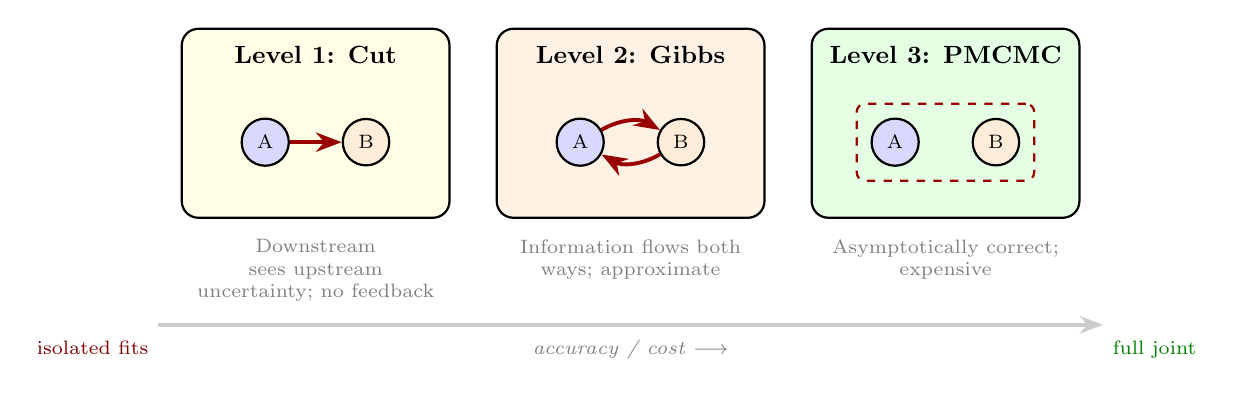
\begin{tikzpicture}[
		scale=0.8,
		lvl/.style={draw, thick, rounded corners=6pt, minimum height=2.4cm, minimum width=3.4cm, align=center},
		circ/.style={draw, thick, circle, minimum size=0.55cm, font=\scriptsize},
		>=Stealth
	]
		% Level 1: Cut
		\node[lvl, fill=yellow!10] (l1) at (0, 0) {};
		\node[font=\small\bfseries, anchor=north] at ([yshift=-4pt]l1.north) {Level 1: Cut};
		\node[circ, fill=blue!15] (a1) at (-0.8, -0.3) {A};
		\node[circ, fill=orange!15] (b1) at (0.8, -0.3) {B};
		\draw[->, line width=1.4pt, red!60!black] (a1) -- (b1);
		\node[font=\scriptsize, text=gray, text width=3.2cm, align=center, anchor=north]
			at ([yshift=-5pt]l1.south) {Downstream sees upstream\\uncertainty; no feedback};

		% Level 2: Gibbs
		\node[lvl, fill=orange!10] (l2) at (5, 0) {};
		\node[font=\small\bfseries, anchor=north] at ([yshift=-4pt]l2.north) {Level 2: Gibbs};
		\node[circ, fill=blue!15] (a2) at (4.2, -0.3) {A};
		\node[circ, fill=orange!15] (b2) at (5.8, -0.3) {B};
		\draw[->, line width=1.4pt, red!60!black] (a2) to[bend left=30] (b2);
		\draw[->, line width=1.4pt, red!60!black] (b2) to[bend left=30] (a2);
		\node[font=\scriptsize, text=gray, text width=3.2cm, align=center, anchor=north]
			at ([yshift=-5pt]l2.south) {Information flows both\\ways; approximate};

		% Level 3: PMCMC
		\node[lvl, fill=green!10] (l3) at (10, 0) {};
		\node[font=\small\bfseries, anchor=north] at ([yshift=-4pt]l3.north) {Level 3: PMCMC};
		\node[circ, fill=blue!15] (a3) at (9.2, -0.3) {A};
		\node[circ, fill=orange!15] (b3) at (10.8, -0.3) {B};
		\node[draw, thick, dashed, rounded corners=3pt, red!60!black,
			  inner sep=5pt, fit=(a3)(b3)] {};
		\node[font=\scriptsize, text=gray, text width=3.2cm, align=center, anchor=north]
			at ([yshift=-5pt]l3.south) {Asymptotically correct;\\expensive};

		% Progression arrow
		\draw[->, line width=1.2pt, gray!40] (-2.5, -3.2) -- (12.5, -3.2);
		\node[font=\scriptsize, text=red!50!black, anchor=north east] at (-2.5, -3.3) {isolated fits};
		\node[font=\scriptsize, text=green!50!black, anchor=north west] at (12.5, -3.3) {full joint};
		\node[font=\scriptsize\itshape, text=gray] at (5, -3.6) {accuracy / cost $\longrightarrow$};
	\end{tikzpicture}

%	\begin{itemize}\itemsep2pt
%		\item { The framework lets you \textbf{choose the level of inferential coupling} for the question you are asking}
%		\item {\tiny \textbf{Diagnostic:} does the posterior change when you allow feedback? If not, the cut was sufficient}
%	\end{itemize}
\end{frame}

% ----------------------------------------------------------------
% "Why Pure Julia?" retired: its diagram and argument are now in the main
% flow, on "Why Hasn't This Been Done?" in Section 2. The four slides below
% are the long-form backing for that slide -- brought over from the old
% Brisbane deck, where they were the "Implications of Root 2" cluster.
% Retitled: this deck does not use the root-1/root-2 numbering.

% ----------------------------------------------------------------







\backupend

\end{document}
